\begin{titlepage}
    \centering
    \vspace*{\fill}

    \vspace*{0.5cm}
    
    \Large% \bfseries
    Capítulo 2

    \vspace*{1cm}

    \Large% \bfseries
    Uso do algoritmo Landtrendr em larga escala no contexto tropical: Um estudo de caso na Mata Atlântica entre os anos de 1985 e 2018

    \vspace*{5cm}

    % \large Eduardo Ribeiro Lacerda

    \vspace*{\fill}
\end{titlepage}

\section{Uso do algoritmo Landtrendr em larga escala no contexto tropical: Um estudo de caso na Mata Atlântica entre os anos de 1985 e 2018}

\begin{abstract}
    abstract
\end{abstract}

\subsection{Introdução}
\hspace{13pt} A disponibilização de forma gratuita de imagens Landsat ao longo dos anos possibilitou um aumento significativo no número de estudos em diversas áreas ao redor do mundo \citep{ZHU2019382, WULDER20122}. Já o surgimento recente de ferramentas de processamento paralelo na nuvem como o Google Earth Engine \citep{GORELICK201718} vem possibilitando agora uma ampliação tanto da área dos estudos quanto também na densidade de cenas, ou seja, na quantidade de imagens Landsat processadas para um único local, o que significa um maior desenvolvimento nas análises temporais.

A incorporação do tempo nas análises espaciais possibilita não só uma maior compreensão dos processos que ocorrem na paisagem como pode ser usado como subsídio para o gerenciamento de recursos e monitoramento de áreas de conservação ou projetos de restauração, estes cada vez mais importantes no contexto geopolítico atual devido principalmente aos efeitos crescentes das mudanças climáticas.

Com o intuito de possibilitar estas análises, algoritmos especializados passaram a ser desenvolvidos principalmente na última década. Podemos citar como exemplo o desenvolvimento de ferramentas como o CCDC \citep{ZHU2014152}, COLD \citep{Cohen2020}, VCT \citep{Huang2010, THOMAS201119} , VerDET \citep{Hughes2017}, EWMACD \citep{Brooks2014}, MIICA \citep{JIN2013159}, ITRA \citep{VOGELMANN201292}, Shapes-NBR \citep{Meyer2013, Moisen2016} e o Landtrendr \citep{KENNEDY20102897, KENNEDY2012117} que tem se mostrado uma das opções mais populares desde sua implementação na plataforma do Google \citep{Kennedy2018}.

No entanto, inicialmente, grande parte destes algoritmos foram desenvolvidos e testados quase sempre em áreas reduzidas e majoritariamente de clima temperado. Ao incorporar ferramentas de processamento de \textit{big data} como o Google Earth Engine, algoritmos como o Landtrendr puderam ser de certa forma expandidos e acabaram viabilizando sua aplicação em áreas de grande extensão, assim como em áreas com diferentes configurações climáticas.

Apesar disso, ainda sim vivemos sob crescente demanda de técnicas que deem conta de forma cada vez mais precisa de projetos de análise e/ou de monitoramento de áreas florestadas devido ao crescente número de projetos de conservação e restauração vinculados muitas vezes à acordos internacionais que impactam diretamente no desenvolvimento econômico dos países. Para além da própria detecção da mudança, se torna cada vez mais necessário a qualificação da detecção, e que as ferramentas utilizadas para a detecção, além de precisas, sejam de fácil implementação, manutenção, validação e possuam preferencialmente baixo requisito computacional.

Uma das áreas sob constante interesse nacional e internacional é o bioma da Mata Atlântica. O interesse pelo bioma é antigo, já que foi a primeira região do Brasil a ser colonizada e também por ser considerado um \textit{hotspot} de biodiversidade \citep{REZENDE2018208}. Devido a sua evolução histórica, é também o bioma mais fragmentando, o que exige, mais do que em outros biomas, um cuidado especial na hora de analisar seus remanescentes. Devido ao efeito da fragmentação, a resolução espacial da análise se torna ainda mais importante já que resoluções mais grosseiras podem levar a uma má interpretação de sua condição ecológica atual, subestimando a quantidade total de floresta. Além disso, devido a sua área extensa, a aplicação de algoritmos de detecção de mudança na região acabam sendo limitados a pequenas regiões, já que são ferramentas que necessitam de alto poder computacional. Este fator dificulta não só possíveis análises quanto principalmente a incorporação de técnicas de detecção de distúrbios baseado em séries temporais em projetos de monitoramento.

Devido a sua importância no contexto nacional, inúmeras análises, acordos e projetos de monitoramento foram e ainda são realizados na região. No entanto, nenhum deles incorporou técnicas de detecção de mudança baseado na segmentação de trajetórias para todo o bioma. Isso significa que para além da detecção de eventos de mudança e sua quantificação em área e cruzamento com suas respectivas classes, ainda existe uma dificuldade na qualificação dessas mudanças. Novas técnicas de análise tem mostrando bons resultados na acurácia das áreas que sofreram algum tipo de interferência e também na adição de informações como a magnitude do evento, ano de detecção, taxa de mudança, entre outros. Informações que atualmente podem ser obtidas, mas somente através de análises posteriores. No entanto, ainda existe dúvida sobre a capacidade de análise de algoritmos como o Landtrendr para áreas tropicais, e principalmente de grande extensão. Seus pontos positivos e negativos não só em relação aos resultados apresentados mas a viabilidade de implementação da técnica para esta quantidade de dados. 

% Vivemos sob a crescente necessidade de desenvolvimento e estabelecimento de técnicas que deem conta da melhor forma possível dos processos de monitoramento de florestas tropicais devido a necessidade de verificação da viabilidade dos projetos de conservação visando a manutenção dos fragmentos restantes e também do suporte necessário a projetos e grandes acordos de restauração de áreas prioritárias \citep{strassburg_strategic_2019}. Parte da busca por uma técnica de monitoramento desses recursos passa por alguns pontos importante. O algoritmo em questão deve poder ser aplicável de forma mais integrada possível em diversos tipos de fitofisionomias e biomas. Além disso, é desejável que o mesmo tenha alta capacidade de adoção pela comunidade científica visando a descentralização do processo de monitoramento e que o algoritmo não possua necessidade de um alto poder processamento que não possa ser acessado pelos mesmos pesquisadores, além de possuir um baixo tempo de implementação devido a restrições legais.

% testar o desempenho do landtrendr em uma área tropical e a viabilidade do mesmo em uma área extensa como o bioma da MA.

Este estudo tem como objetivo buscar um melhor entendimento da capacidade do algoritmo Landtrendr na detecção das dinâmicas ocorridas ao longo de mais de três décadas para todo o bioma da Mata Atlântica considerando suas principais fitofisionomias. Foram analisadas áreas de vegetação estacional semi-decidual, vegetação ombrófila densa e também áreas de vegetação ombrófila mista. Áreas com predominância de vegetação de estepe, savânica, mangue, além de áreas altamente antropisadas foram excluídas da análise. 

% Adaptação do Mapa de Limites de Biomas 1:5.000.000 produzido pelo IBGE, refinado a partir do Mapa de Limites do território 1:250.000 (IBGE) e o mapa de fitofisionomias 1:1.000.000 (IBGE).

A escolha deste algoritmo se deu pelo mesmo ter obtido resultados mais interessantes quando comparado a outras técnicas \citep{Saxena2018} e devido a sua recente implementação na plataforma Google Earth Engine \citep{Kennedy2018}, o que facilitou sua aplicação a uma área tão grande como a deste bioma. 

\subsection{Materiais e Métodos}
\subsubsection{Área de estudo}
\hspace{13pt} O estudo abrange toda a área do bioma da Mata Atlântica dentro do território brasileiro (Figura \ref{fig:mata_atlantica}), que possui atualmente uma área total de aproximadamente 1.1 Mkm2 ou 110 Mha. O bioma está presente em 15 estados brasileiros e é onde se localiza grande parte da atividade econômica e população do pais. Atualmente, vivem na Mata Atlântica cerca de 72\% da população brasileira, o que em parte explica o fato de hoje apenas cerca de 28\% \citep{REZENDE2018208} de sua cobertura natural ter persistido.. O bioma ainda possui 75,6\% das espécies ameaçadas e endêmicas do Brasil, o que o torna um dos mais prioritários para conservação no país. Além disso, estima-se que entre 43\% e 45\% do total de espécies de plantas e vertebrados sejam restritas a esse bioma \citep{scarano2014}. O número elevado de espécies no bioma o coloca como a quinta área mais ameaçada e rica em espécies endêmicas do Mundo. No total são 1.361 espécies, sendo 261 espécies de mamíferos, 620 de aves, 200 de répteis e 280 de anfíbios. Das 1.361, 567 só ocorrem neste bioma \citep{IBGE_BIOMAS}.

\begin{figure}[h!]
    \centering
    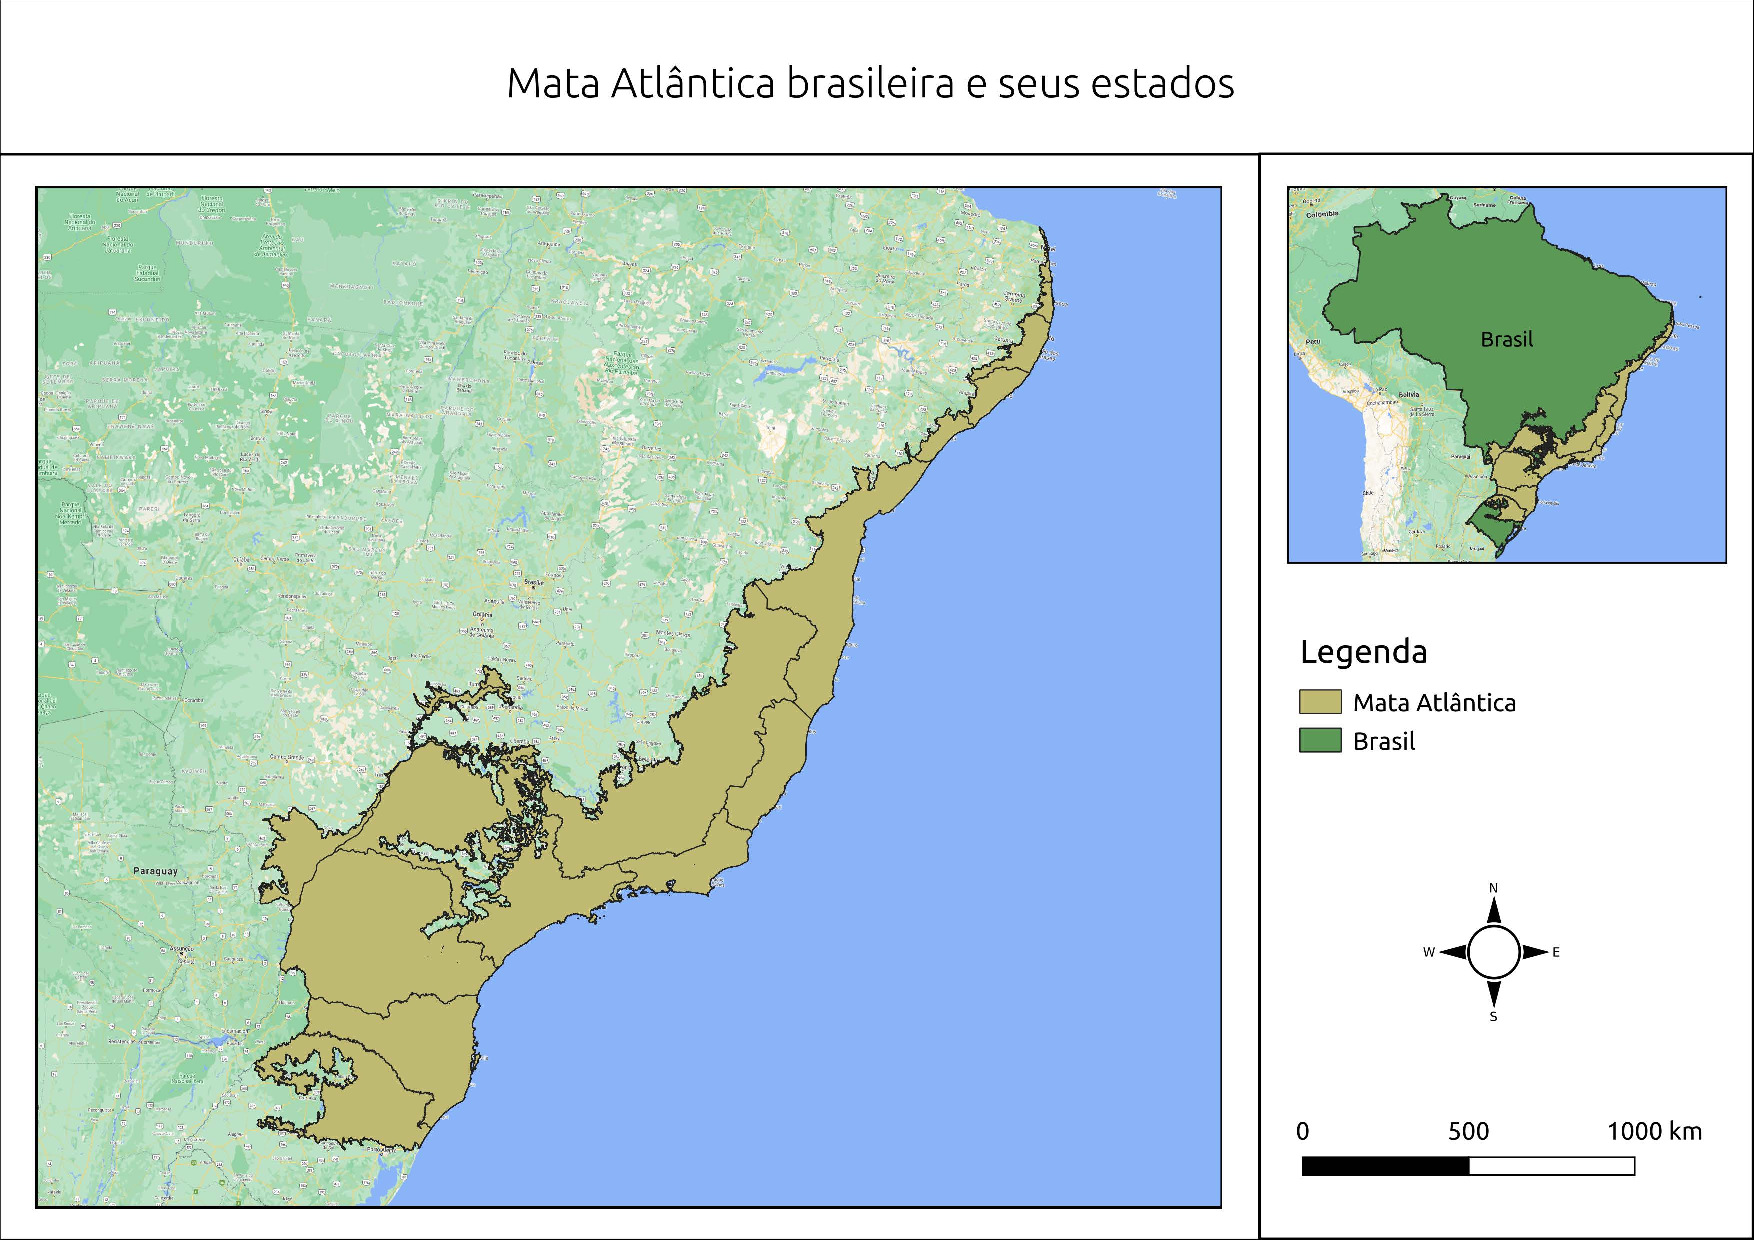
\includegraphics[scale=.5]{images/mata_atlantica.pdf}
    \caption{Área de Estudo - Mata Atlântica brasileira}
    \label{fig:mata_atlantica}
\end{figure}

Na época da chegada dos portugueses no Brasil, a Mata Atlântica cobria cerca de 1,5 milhões de quilômetros quadrados (incluindo ecótonos), estendendo-se ao longo de 3 mil quilômetros da costa brasileira - do Rio Grande do Sul ao Rio Grande do Norte - e penetrando pelo interior, cruzando São Paulo, Minas Gerais e Mato Grosso do Sul até as fronteiras da Argentina e do Paraguai \citep{scarano2014}. Cerca de 500 anos depois, esse extenso e representativo bioma abriga mais de 100 milhões de pessoas, cerca de 1/4 das quais ainda vivem na pobreza \citep{scarano2014}.

Segundo o projeto Mapbiomas \citep{Souza2019}, a área total de florestas no bioma em 1985 era de mais de 30 Mha e em 2018 de 28 Mha. Já a área de florestas que não sofreram mudanças significativas (pseudo-invariantes) durante o período de 1985 até 2018 foi de aproximadamente 21.4 Mha. Deste total, somente  30\% da vegetação nativa remanescente está protegida legalmente através de unidades de conservação.

% Apesar dos importantes avanços obtidos nesta agenda na última década – como a restauração de aproximadamente 1,4 milhões de hectares entre 2011 e 2020 – muito ainda precisa ser feito \citep{CROUZEILLES2019}

\subsubsection{Dados de entrada}
\hspace{13pt} Para o mapeamento do bioma consideramos um intervalo anual que compreendeu todos os anos de 1985 até 2018 utilizando imagens do satélite Landsat das séries 5, 7 e 8. A escolha desse período de análise se deu por conta do início da captura de dados em 1 de março de 1984 pelo satélite Landsat 5 e consequente disponibilidade de dados pela comunidade científica para o mesmo período, o que facilitou a verificação e validação dos resultados. Para cobrir todos os 110 Mha do bioma foi necessário a compilação e processamento de 88 cenas Landsat, cada cena cobrindo os 33 anos da análise com cerca de 23 imagens por ano, o que dá algo em torno de aproximadamente 67 mil imagens, o que representa quase 2.5x toda a quantidade de imagens Landsat utilizada em estudos no continente sul americano nos últimos 50 anos \citep{Hemati2021}. Se considerarmos que cada uma dessas imagens utilizadas possui pelo menos 7 bandas, chegamos a um cubo multidimensional de quase meio milhão de bandas. Um processamento que sem dúvidas só seria possível com o advento das tecnologias já citadas.

Todas as imagens utilizadas são da coleção \emph{surface reflectance}, o que significa que já possuem correção geométrica, radiométrica e possuem valor físico referente a superfície terrestre. Além disso, as imagens passaram por processo de harmonização para evitar acúmulo de ruídos e também de remoção de nuvens e sombras. Todos os processamentos para a composição das séries temporais foram feitos utilizando funções internas do próprio Landtrendr, o que facilitou em muito toda a etapa de preparação dos dados.

\subsubsection{Método de análise}
\hspace{13pt} A análise das trajetórias foi feita utilizando o algoritmo Landtrendr em sua versão para a plataforma Google Earth Engine (GEE) \citep{Kennedy2018}. A principal vantagem da implementação do algoritmo no GEE em relação a sua versão original em ENVI/IDL está na possibilidade de sua aplicação em áreas extensas com um tempo de pré-processamento e análise em si muito menores, o que possibilita sua aplicação em contextos anteriormente inviáveis. O ganho de tempo não está somente no tempo de processamento do algoritmo em si, como também na eliminação de grande parte dos desafios técnicos relacionados ao processamento dos dados de entrada presentes em sua implementação clássica. No entanto, apesar do ganho significativo no tempo de processamento, o Landtrendr para o GEE também apresenta algumas limitações quando comparado a sua versão em original em IDL. Uma das maiores está na limitação na extensão da análise para apenas uma imagem Landsat por vez. A plataforma apresentou erros sistemáticos quando requisitada para processar análises para toda a Mata Atlântica de uma só vez, ou para áreas que abrangiam vários estados, por exemplo. Com isso, o processamento teve de ser feito em etapas. 

As etapas tiveram de ser divididas por cenas Landsat, neste caso, 88 cenas (Figura \ref{fig:pathrow_centroids}). Como o resultado do algoritmo é dado de forma separada por cena, foi necessário juntar todas as camadas geradas. Devido a ruídos presentes nas bordas das imagens Landsat e a sobreposição natural entre imagens diferentes, nem todos os pixels presentes nas bordas apresentaram resultados similares. Juntar todos as 88 camadas de resultados em uma se tornou um desafio e só foi possível através da criação de polígonos de voronoi \citep{Okabe}, o que possibilitou utilizarmos somente as áreas mais próximas do centro das camadas geradas pelo algoritmo (Figura \ref{fig:voronoi_example}).

\begin{figure}[H]
    \centering
    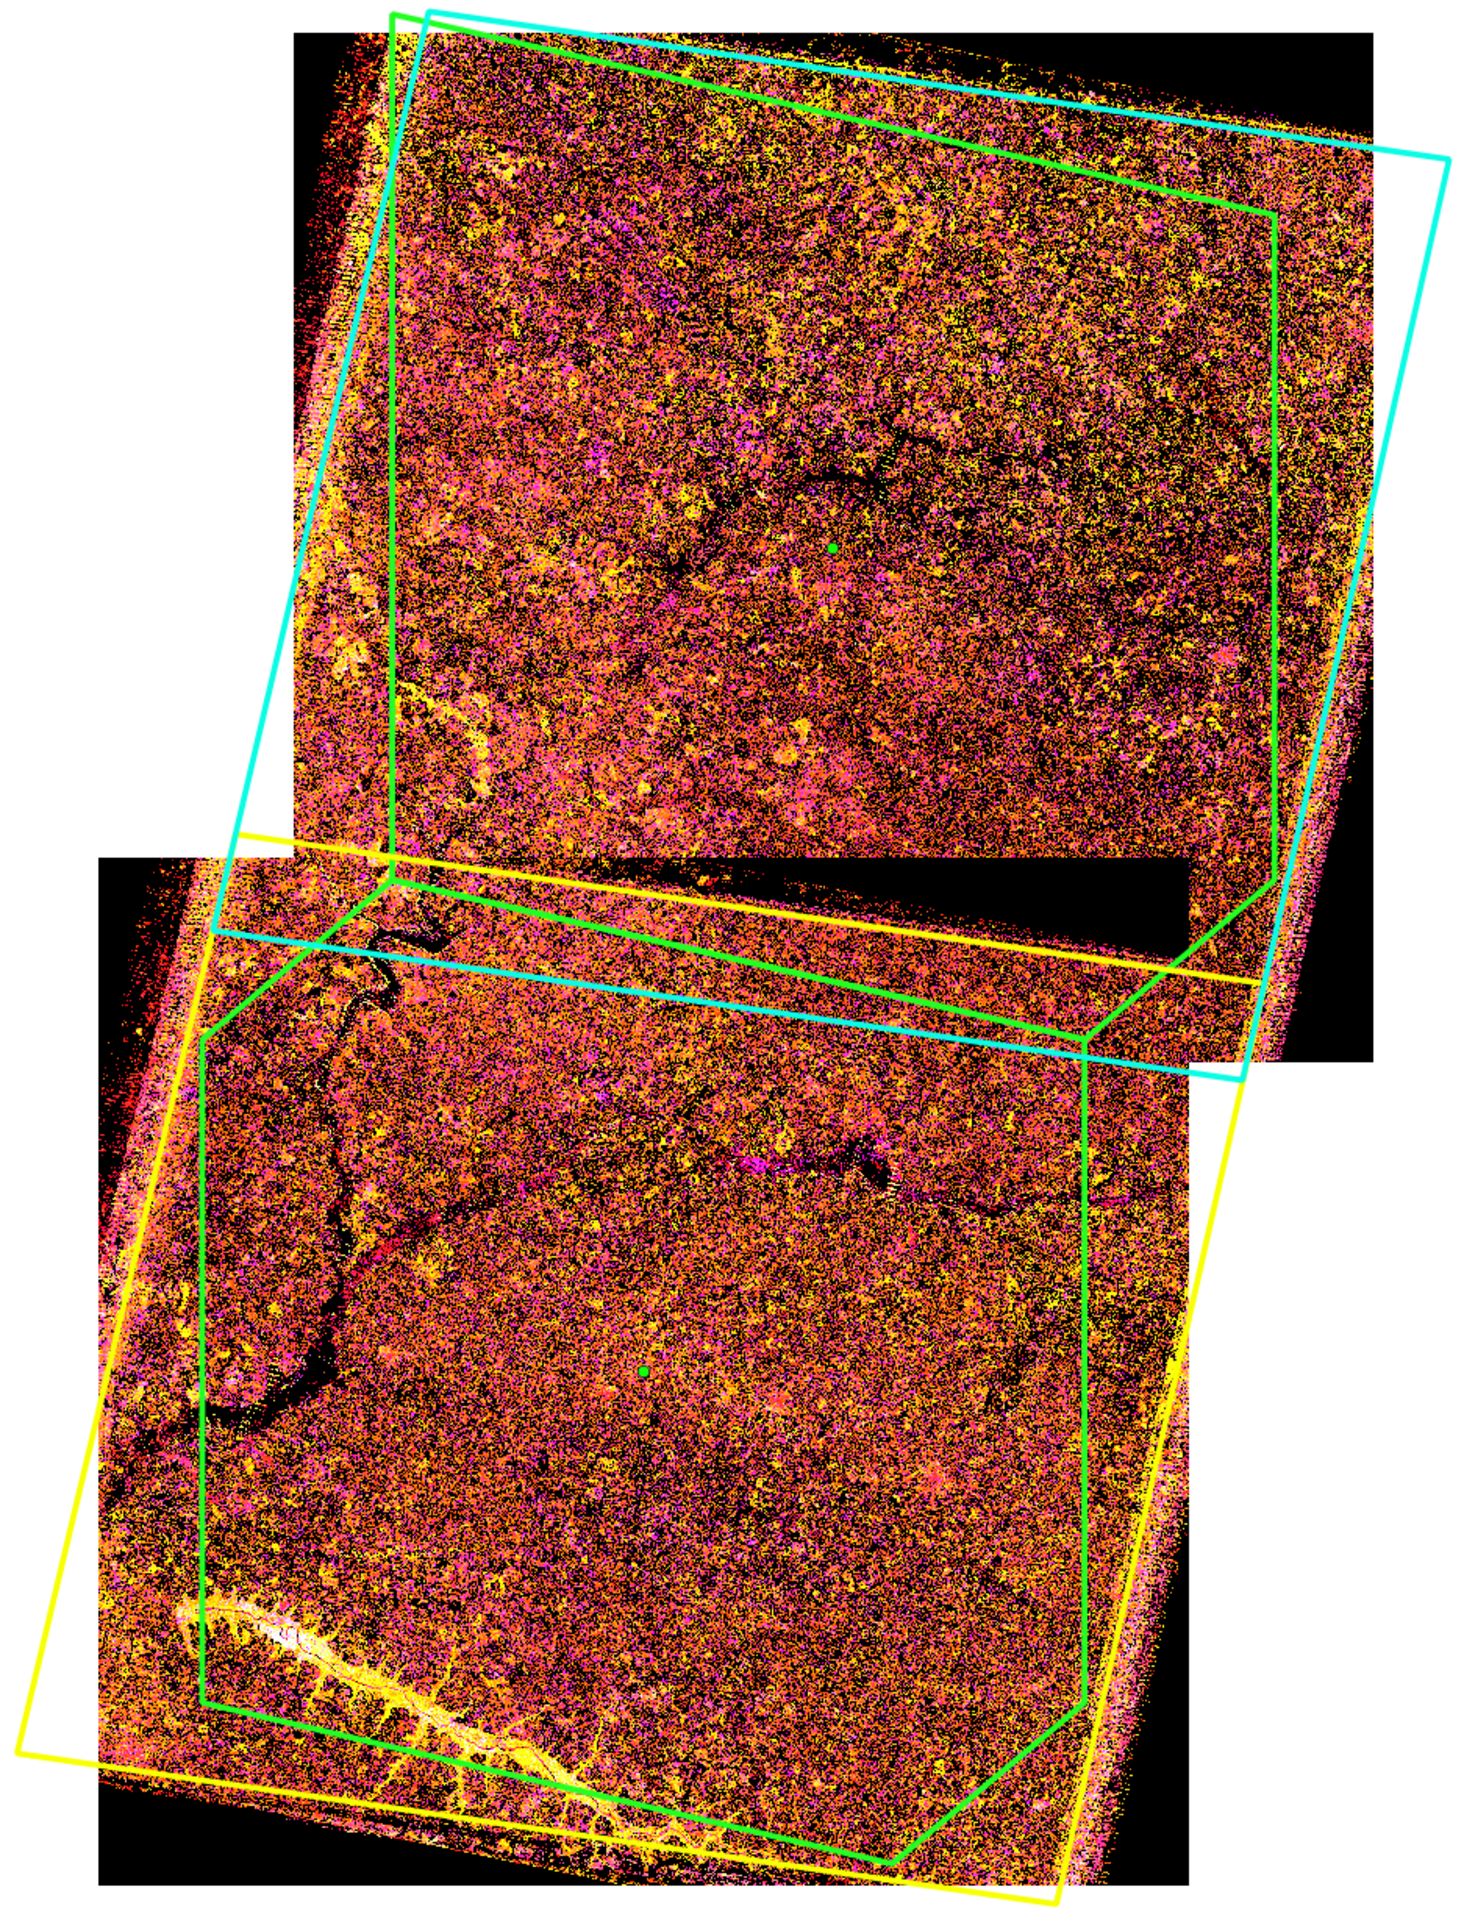
\includegraphics[scale=.5]{images/voronoi_example.pdf}
    \caption{No centro das duas imagens podemos ver os centroides em verde, assim como os polígonos de voronoi na mesma cor. Já em ciano e amarelo, podemos observar os polígonos envolventes para as cenas Landsat 222/73 e 222/74. As imagens de fundo são compostas pela composição das seis bandas geradas pelo Landtrendr para as duas cenas. É possível ver a presença de sobreposição entre os dois resultados a partir dos retângulos envolventes do satélite e também de sobreposição nos polígonos de voronoi.}
    \label{fig:voronoi_example}
\end{figure}

\begin{figure}[h!]
    \centering
    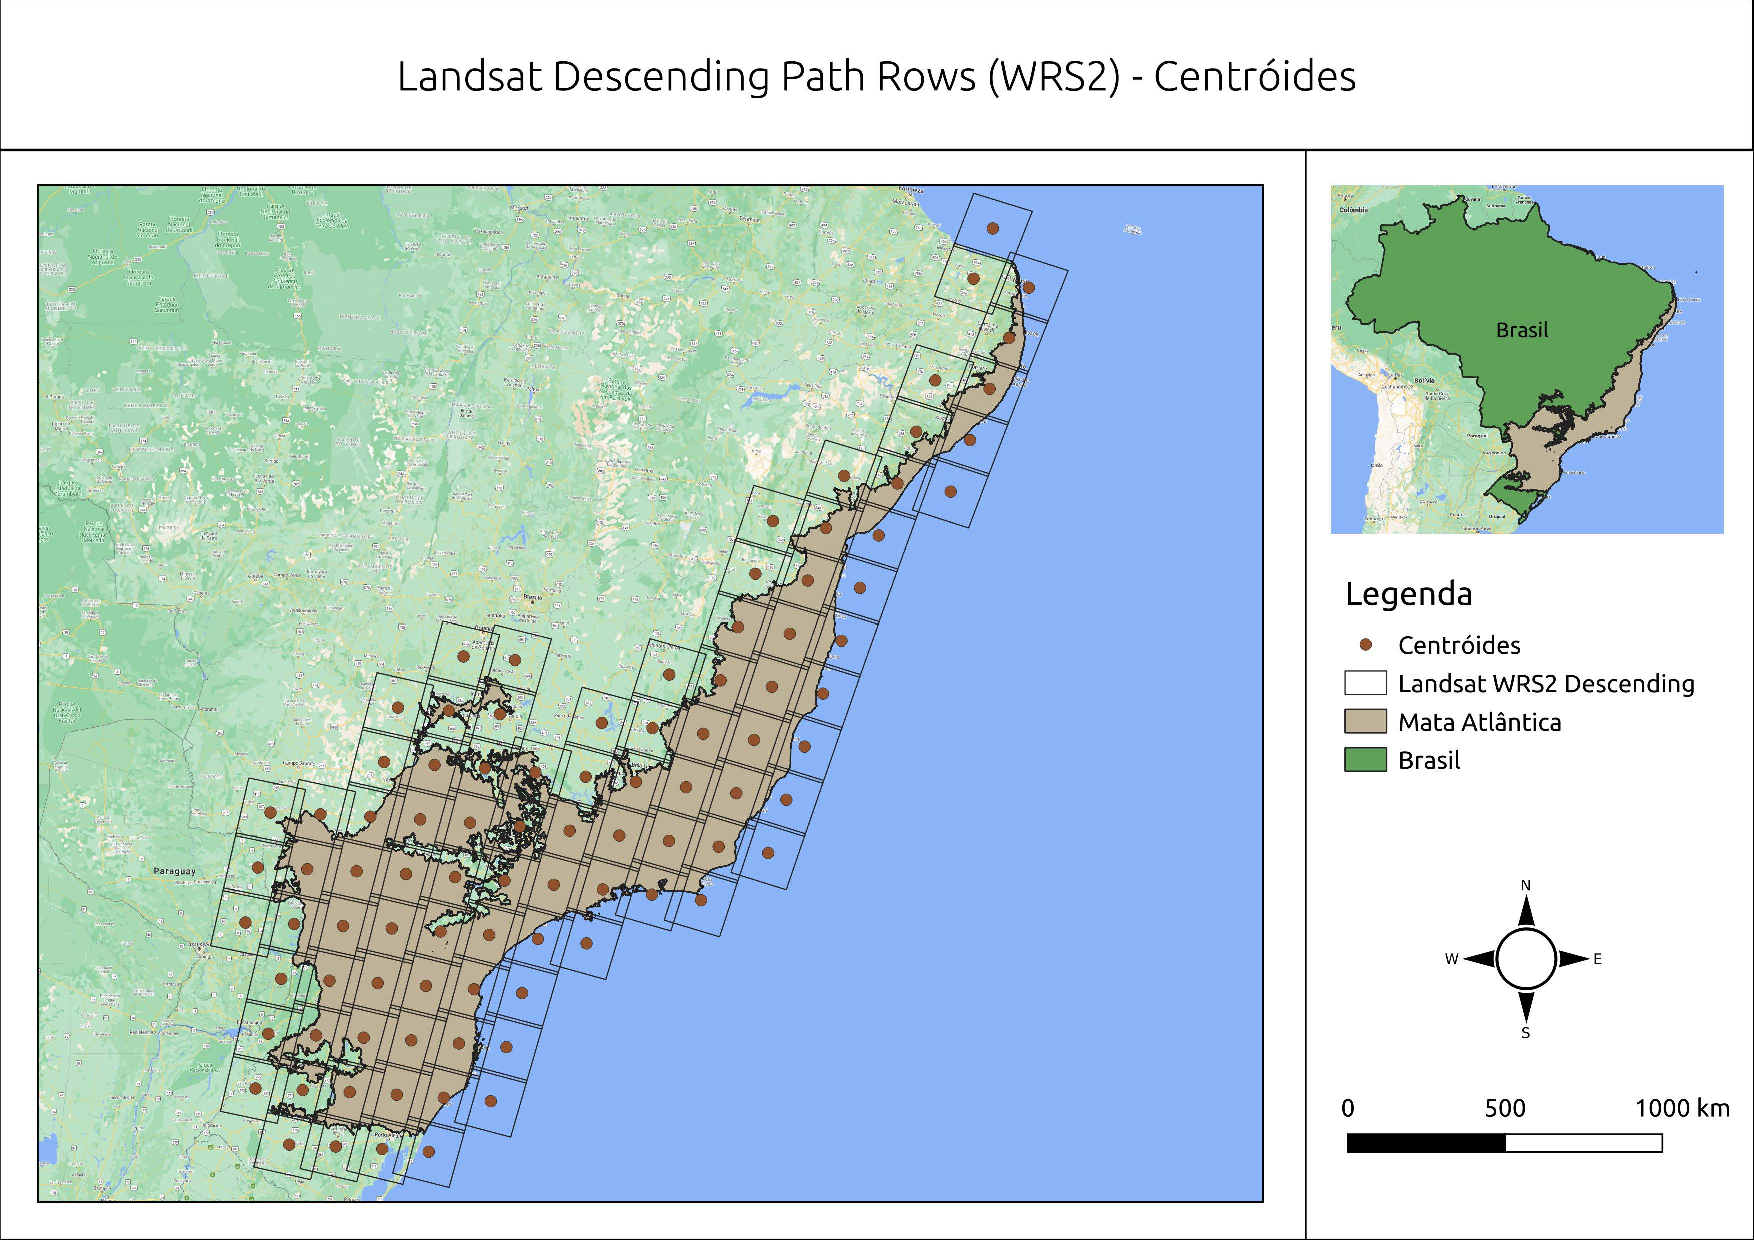
\includegraphics[scale=.5]{images/ma_pathrow_centroids.pdf}
    \caption{Pathrows das imagens Landasat e seus respectivos centróides que foram utilizados para delimitar as cenas a serem processadas pelo algoritmo}
    \label{fig:pathrow_centroids}
\end{figure}

Os polígonos de voronoi foram gerados através da extração dos centroides dos polígonos delimitadores das cenas Landsat e posteriormente utilizados para a criação dos polígonos com as áreas centrais (Figura \ref{fig:voronoi_ma}). Após a geração dos polígonos de voronoi, os mesmos foram utilizados para recortar os resultados de forma a limpar possíveis sobreposições. Após o recorte, todas as imagens foram agregadas para toda extensão do bioma e separadas banda a banda para análise posterior.

\begin{figure}[H]
    \centering
    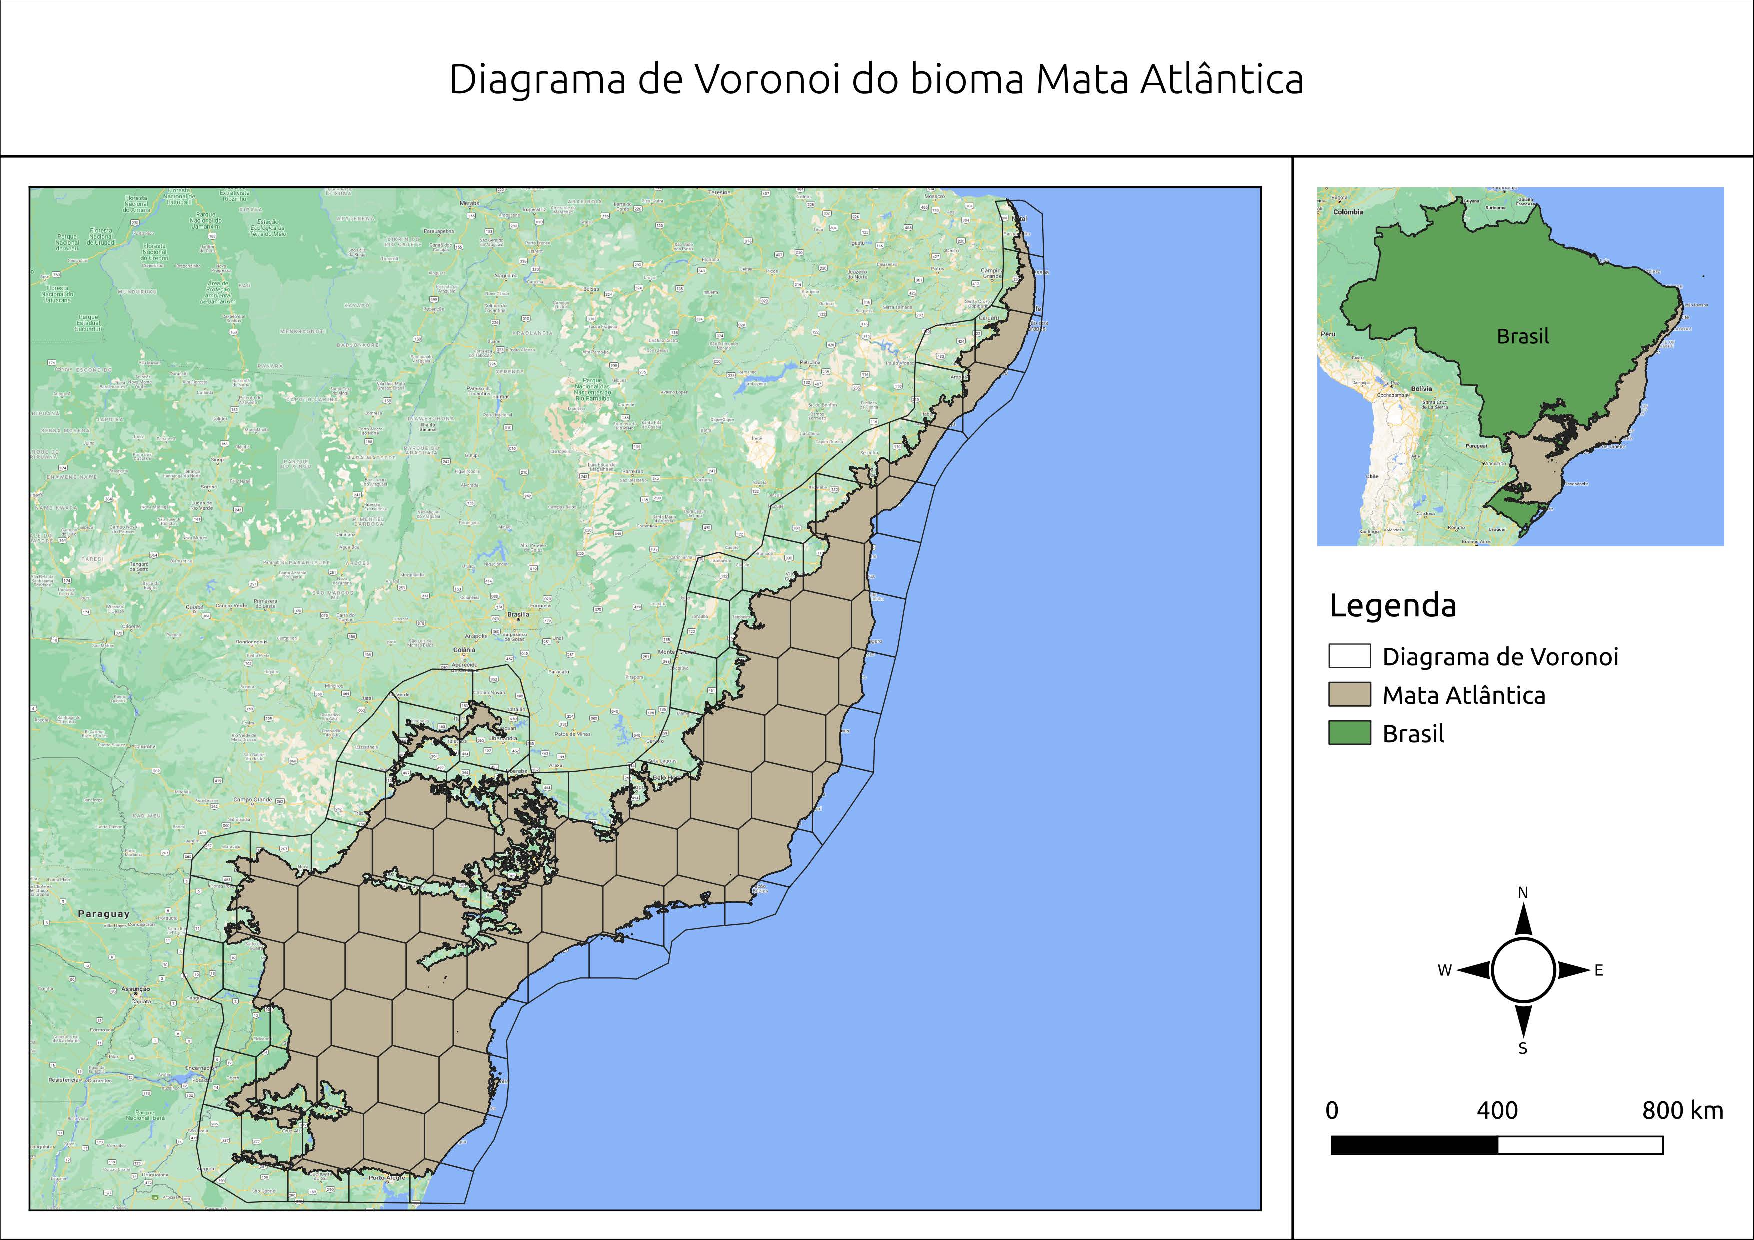
\includegraphics[scale=.5]{images/voronoi_mata_atlantica.pdf}
    \caption{Diagrama de Voronoi criado a partir dos centróides.}
    \label{fig:voronoi_ma}
\end{figure}

O algoritmo Landtrendr trabalha analisando os valores pixel a pixel para toda a composição de imagens visando criar segmentos e assim identificar trajetórias (Figura \ref{fig:landtrendr_graph}). O algoritmo pode gerar métricas tanto para distúrbios de perda como de ganho, além de detectar mudanças que ocorreram de forma lenta ou rápida, possibilitando também o cálculo da duração de eventos segmentados previamente gerando dados contínuos, discretos, assim como a duração e o ano da detecção. Podemos analisar, portanto, a história do pixel em questão, neste caso, sob uma perspectiva meso-escalar das florestas de Mata Atlântica. Para realizar o processo de segmentação temporal o algoritmo pode utilizar tanto uma banda padrão do satélite como algum índice espectral. Alguns índices já bem estabelecidos já estão implementados na ferramenta como o NDVI (\textit{Normalized Difference Vegetation Index}), o EVI (\textit{Enhanced vegetation index}), o NDMI (\textit{Normalized Difference Moisture Index}) e o NBR (\textit{Normalized Burn Ratio}). É possível também utilizar uma das próprias bandas do satélite para realizar as análises, como a banda do vermelho ou o SWIR (\textit{Short-wave infrared}). 

% Apesar de bandas como o NBR e NDMI mostrarem bons resultados em regiões de floresta temperada, testes realizados em florestas tropicais mostraram que índices como o NDVI apresentam resultados superiores \citep{zebende2019}. 
% Sendo assim, para este estudo, o processo de segmentação temporal foi realizado utilizando o NDVI como banda base.
% Adicionar todo o conteúdo sobre o CSNR (Change Signal to Noise Ratio).

\begin{figure}[h!]
    \centering
    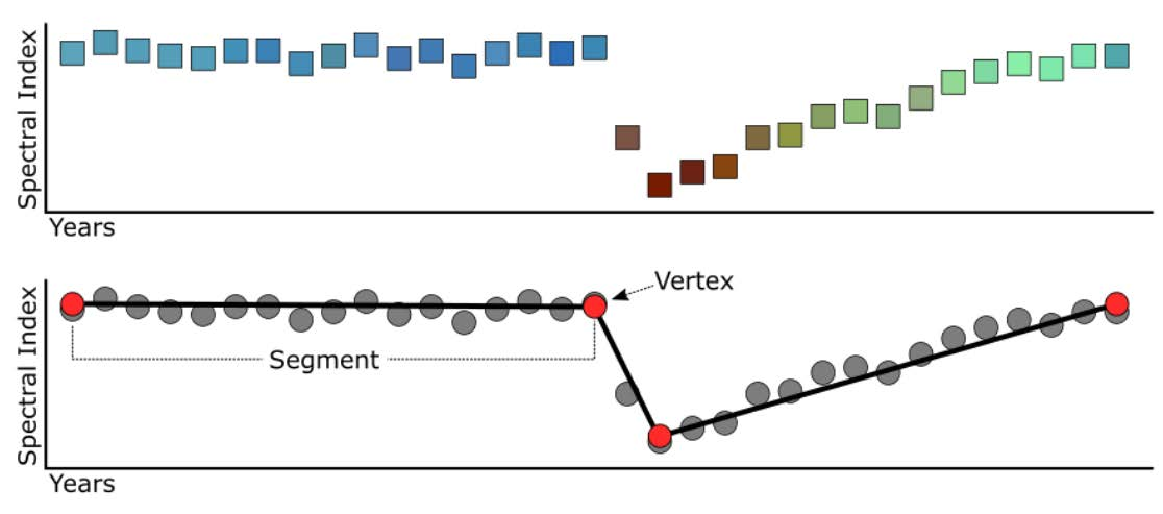
\includegraphics[scale=.8]{images/landtrendr_graphic.pdf}
    \caption{Segmentação temporal do pixel pelo algoritmo Landtrendr. \\ Fonte: Documentação oficial}
    \label{fig:landtrendr_graph}
\end{figure}

\subsubsection{Escolha da banda ou índice a ser analisado}

A escolha do índice a ser utilizado é parte importante do processo já que essa escolha pode influenciar na precisão do processo de identificação das mudanças de acordo com o que se está tentando detectar. O índice NBR, tradicional no monitoramento de queimadas vem mostrando excelentes resultados na detecção de mudanças em áreas de florestas temperadas, com resultados superiores a índices mais tradicionais como o próprio NDVI ou o EVI.

Em áreas tropicais, o uso de índices com o NDVI ainda é predominante \citep{zebende2019, FRAGAL2016}, mas devido a variabilidade na qualidade dos resultados de acordo com a banda ou índice utilizado, o algoritmo fornece como uma das camadas resultantes de cada análise realizada uma banda extra chamada CSNR (\textit{Change Signal to Noise Ratio}), que oferece uma métrica para entender qual banda pode ser ideal para cada tipo de região estudada. Como a mesma só pode ser gerada após a execução do algoritmo, é recomendado que o algoritmo seja primeiro executado para uma mesma área teste diversas vezes utilizando bandas e índices diferentes para cada rodada. Bandas/índices que obtiverem maior valor médio geral na camada CSNR possuem menor quantidade de erro associada ao processo de detecção de mudanças.

Sendo assim, o teste com a banda CSNR foi realizado para as 13 bandas/índices (Azul, Verde, Vermelho, NIR, SWIR, Tasseled Cap Brightness/Greenness/Wetness, NBR, NBRz, NDVI, EVI e NDMI) presentes no algoritmo para cada uma das fitofisionomias estudadas no bioma neste estudo (Tabela \ref{tab:csnr_results}). 


\begin{table}[h!]
    \centering
    \rowcolors{2}{red!50!yellow!30}{green!40!yellow!10}
    % \footnotesize
    \begin{tabular}{| c | c | c| c | c |}
    \hline
            Camada & Est. Semidecidual & Omb. Mista & Omb. Densa & Média \\
            SWIR & 2.53 & \textbf{3.47} & \textbf{3.00} & \textbf{3.00} \\
            Vermelho & 2.49 & 3.25 & 2.93 & 2.89 \\
            TCW & 2.40 & 3.26 & 2.95 & 2.87 \\
            Verde & 2.42 & 3.16 & 2.76 & 2.78 \\
            TCB & \textbf{2.58} & 3.05 & 2.66 & 2.77 \\
            EVI & 2.56 & 2.82 & 2.87 & 2.75 \\
            NDMI & 2.27 & 2.86 & 2.98 & 2.70 \\
            NDVI & 2.40 & 2.85 & 2.86 & 2.70 \\
            NBR & 2.27 & 2.90 & 2.81 & 2.66 \\
            NBRz & 2.25 & 2.88 & 2.81 & 2.65 \\
            TCG & 2.05 & 2.19 & 2.53 & 2.26 \\
            NIR & 2.06 & 2.17 & 2.31 & 2.18 \\
            Azul & 1.92 & 2.36 & 2.19 & 2.16 \\
    \hline
    \end{tabular}
    \caption{Mediana dos valores da camada CSNR para cada banda/índice em cada fitofisionomia (Estacional Semidecidual, Ombrófila Mista e Ombrófila Densa). A última coluna representa a média geral da banda/índice considerando todas as medianas obtidas em todas as fitofisionomias.}
    \label{tab:csnr_results}
\end{table}

Podemos observar que de forma geral os melhores resultados se concentraram nas regiões de floresta ombrófila com uma maior quantidade de ruído nas regiões estacionais, resultado de certa forma já esperado devido a maior interferência estrutural devido ao ciclo das estações. Mesmo analisando composições anuais, podemos perceber que existe interferência no valor mediano em regiões estacionais suficiente para influenciar na geração de ruídos. Apesar disso, o acréscimo de ruídos nas regiões estacionais não impactou o resultado final a ponto de influenciar a acurácia global de forma significativamente negativa.

Quanto aos índices disponíveis, nenhum apresentou resultado superior para todas as fitofisionomias. Para as áreas de vegetação ombrófila, a banda do SWIR apresentou o melhor resultado tanto nas áreas mistas quanto densas. Já nas áreas semideciduais, o melhor resultado se deu com os valores de bilho do Tasseled Cap, seguido do EVI. O tradicional NDVI obteve um resultado geral mediano, tecnicamente empatado com o NDMI. Já na média geral, foi o SWIR que obteve melhor resultado. O NBR, índice recorrente em trabalhos aplicados a áreas temperadas não se saiu tão bem em ambientes tropicais, mas se posicionando logo abaixo do NDVI.

Apesar desses resultados iniciais, um novo teste foi realizado. Desta vez, uma nova área de teste dentro de florestas ombrófilas densas foi adicionada com o intuito de entender se os resultados obtidos se manteriam similares entre fitofisionomias semelhantes. A área escolhida foi dentro da Bacia Hidrográfica do Rio Sâo João (BHRSJ). Através do novo teste, foi possível observar que houve grande variabilidade na escolha dos melhores índices/bandas mesmo em regiões similares. Desta vez, a banda do vermelho obteve o melhor resultado, seguido do NDVI, o que fez a média geral do índice normalizado subir (Tabela \ref{tab:csnr_results_com_bhrsj}).


\begin{table}[h!]
    \centering
    \rowcolors{2}{red!50!yellow!30}{green!40!yellow!10}
    % \footnotesize
    \begin{tabular}{| c | c | c | c| c | c |}
    \hline
            Camada & BHRSJ & Est. Semidecidual & Omb. Mista & Omb. Densa & Média \\
            SWIR & 3.09 & 2.53 & \textbf{3.47} & \textbf{3.00} & \textbf{3.02} \\
            Vermelho & \textbf{3.35} & 2.49 & 3.25 & 2.93 & 3.00 \\
            TCW & 3.00 & 2.40 & 3.26 & 2.95 & 2.90 \\
            Verde & 3.15 & 2.42 & 3.16 & 2.76 & 2.87 \\
            NDVI & 3.25 & 2.40 & 2.85 & 2.86 & 2.84 \\
            TCB & 2.86 & \textbf{2.58} & 3.05 & 2.66 & 2.79 \\
            NDMI & 3.00 & 2.27 & 2.86 & 2.98 & 2.78 \\
            EVI & 2.85 & 2.56 & 2.82 & 2.87 & 2.77 \\
            NBRz & 2.94 & 2.25 & 2.88 & 2.81 & 2.72 \\
            NBR & 2.88 & 2.27 & 2.90 & 2.81 & 2.71 \\
            TCG & 2.93 & 2.05 & 2.19 & 2.53 & 2.43 \\
            NIR & 2.68 & 2.06 & 2.17 & 2.31 & 2.31 \\
            Azul & 2.40 & 1.92 & 2.36 & 2.19 & 2.22 \\
    \hline
    \end{tabular}
    \caption{Mediana dos valores da camada CSNR para cada banda/índice em cada fitofisionomia (Estacional Semidecidual, Ombrófila Mista e Ombrófila Densa). A última coluna representa a média geral da banda/índice considerando todas as medianas obtidas em todas as fitofisionomias.}
    \label{tab:csnr_results_com_bhrsj}
\end{table}

Observando os resultado obtidos, entende-se que a escolha do índice ou banda a ser utilizada para a análise dependa muito mais do que se busca detectar do que necessariamente a camada com maior valor obtido pela banda CSNR. Além disso, para áreas de estudo extensas, é possível que não exista coerência entre os resultados para áreas em teoria similares. Essas diferenças acabam reforçando ainda mais a preocupação com o uso de bandas e índices já conhecidos e estudados anteriormente de acordo com cada contexto.

Entende-se também ser possível utilizar índices que obtiveram o melhor resultado para cada caso como o do SWIR no caso de florestas ombrófilas e do TCB para áreas de florestas estacionais semideciduais para estudos que envolvam áreas mais restritas. Outra possibilidade analisada através dos resultados obtidos é a utilização de uma combinação de bandas/índices diferentes para áreas extensas que envolvam uma ou mais fitofisionomias. No entanto, é necessário pensar no custo-benefício dessa escolha, já que a mesma envolveria uma série de testes e processos fragmentados, elevando significativamente o tempo total de execução e viabilidade do estudo. 

Neste trabalho, o NDVI foi utilizado para a detecção de mudanças para toda a extensão do bioma. Esta escolha se deu com o objetivo de testar o desempenho final do resultados buscando entender se a escolha de um único índice, principalmente um tradicional com o NDVI, pode gerar resultados satisfatórios para áreas extensas de floresta tropical. A utilização de uma única camada tem ainda como objetivo facilitar o processo de interpretação geral e de contribuir com análises comparativas entre fitofisionomias. A escolha do índice significa apenas uma etapa do processo, sendo necessário pensar a escolha de outros parâmetros.

Tanto os resultados para o cenário de perda quanto de ganho foram gerados com o objetivo de detectar supressões e processos de degradação, assim como de restauração e regeneração da floresta (Figura \ref{fig:flowchart_medologia_landtrendr}). Para este estudo, o Landtrendr foi aplicado utilizando todos seus parâmetros padrões. Os tipos de eventos (perda ou ganho) foram organizados de acordo com seu maior evento/segmento (\textit{Greatest Loss / Greatest Gain}).

Posterior aos resultados obtidos pelo algoritmo, toda a etapa de pós-processamento dos dados gerados no GEE foi desenvolvida em ambiente \textit{offline} utilizando ferramentas \textit{open source} como o QGIS \citep{QGIS_software}, GDAL \citep{gdal}, e a linguagem de programação R \citep{Rsoftware}, utilizando os pacotes Raster \citep{raster}, Terra \cite{terra}, gdalUtils \citep{gdalutils} e MLR \citep{mlr}.

\begin{figure}[H]
    \centering
    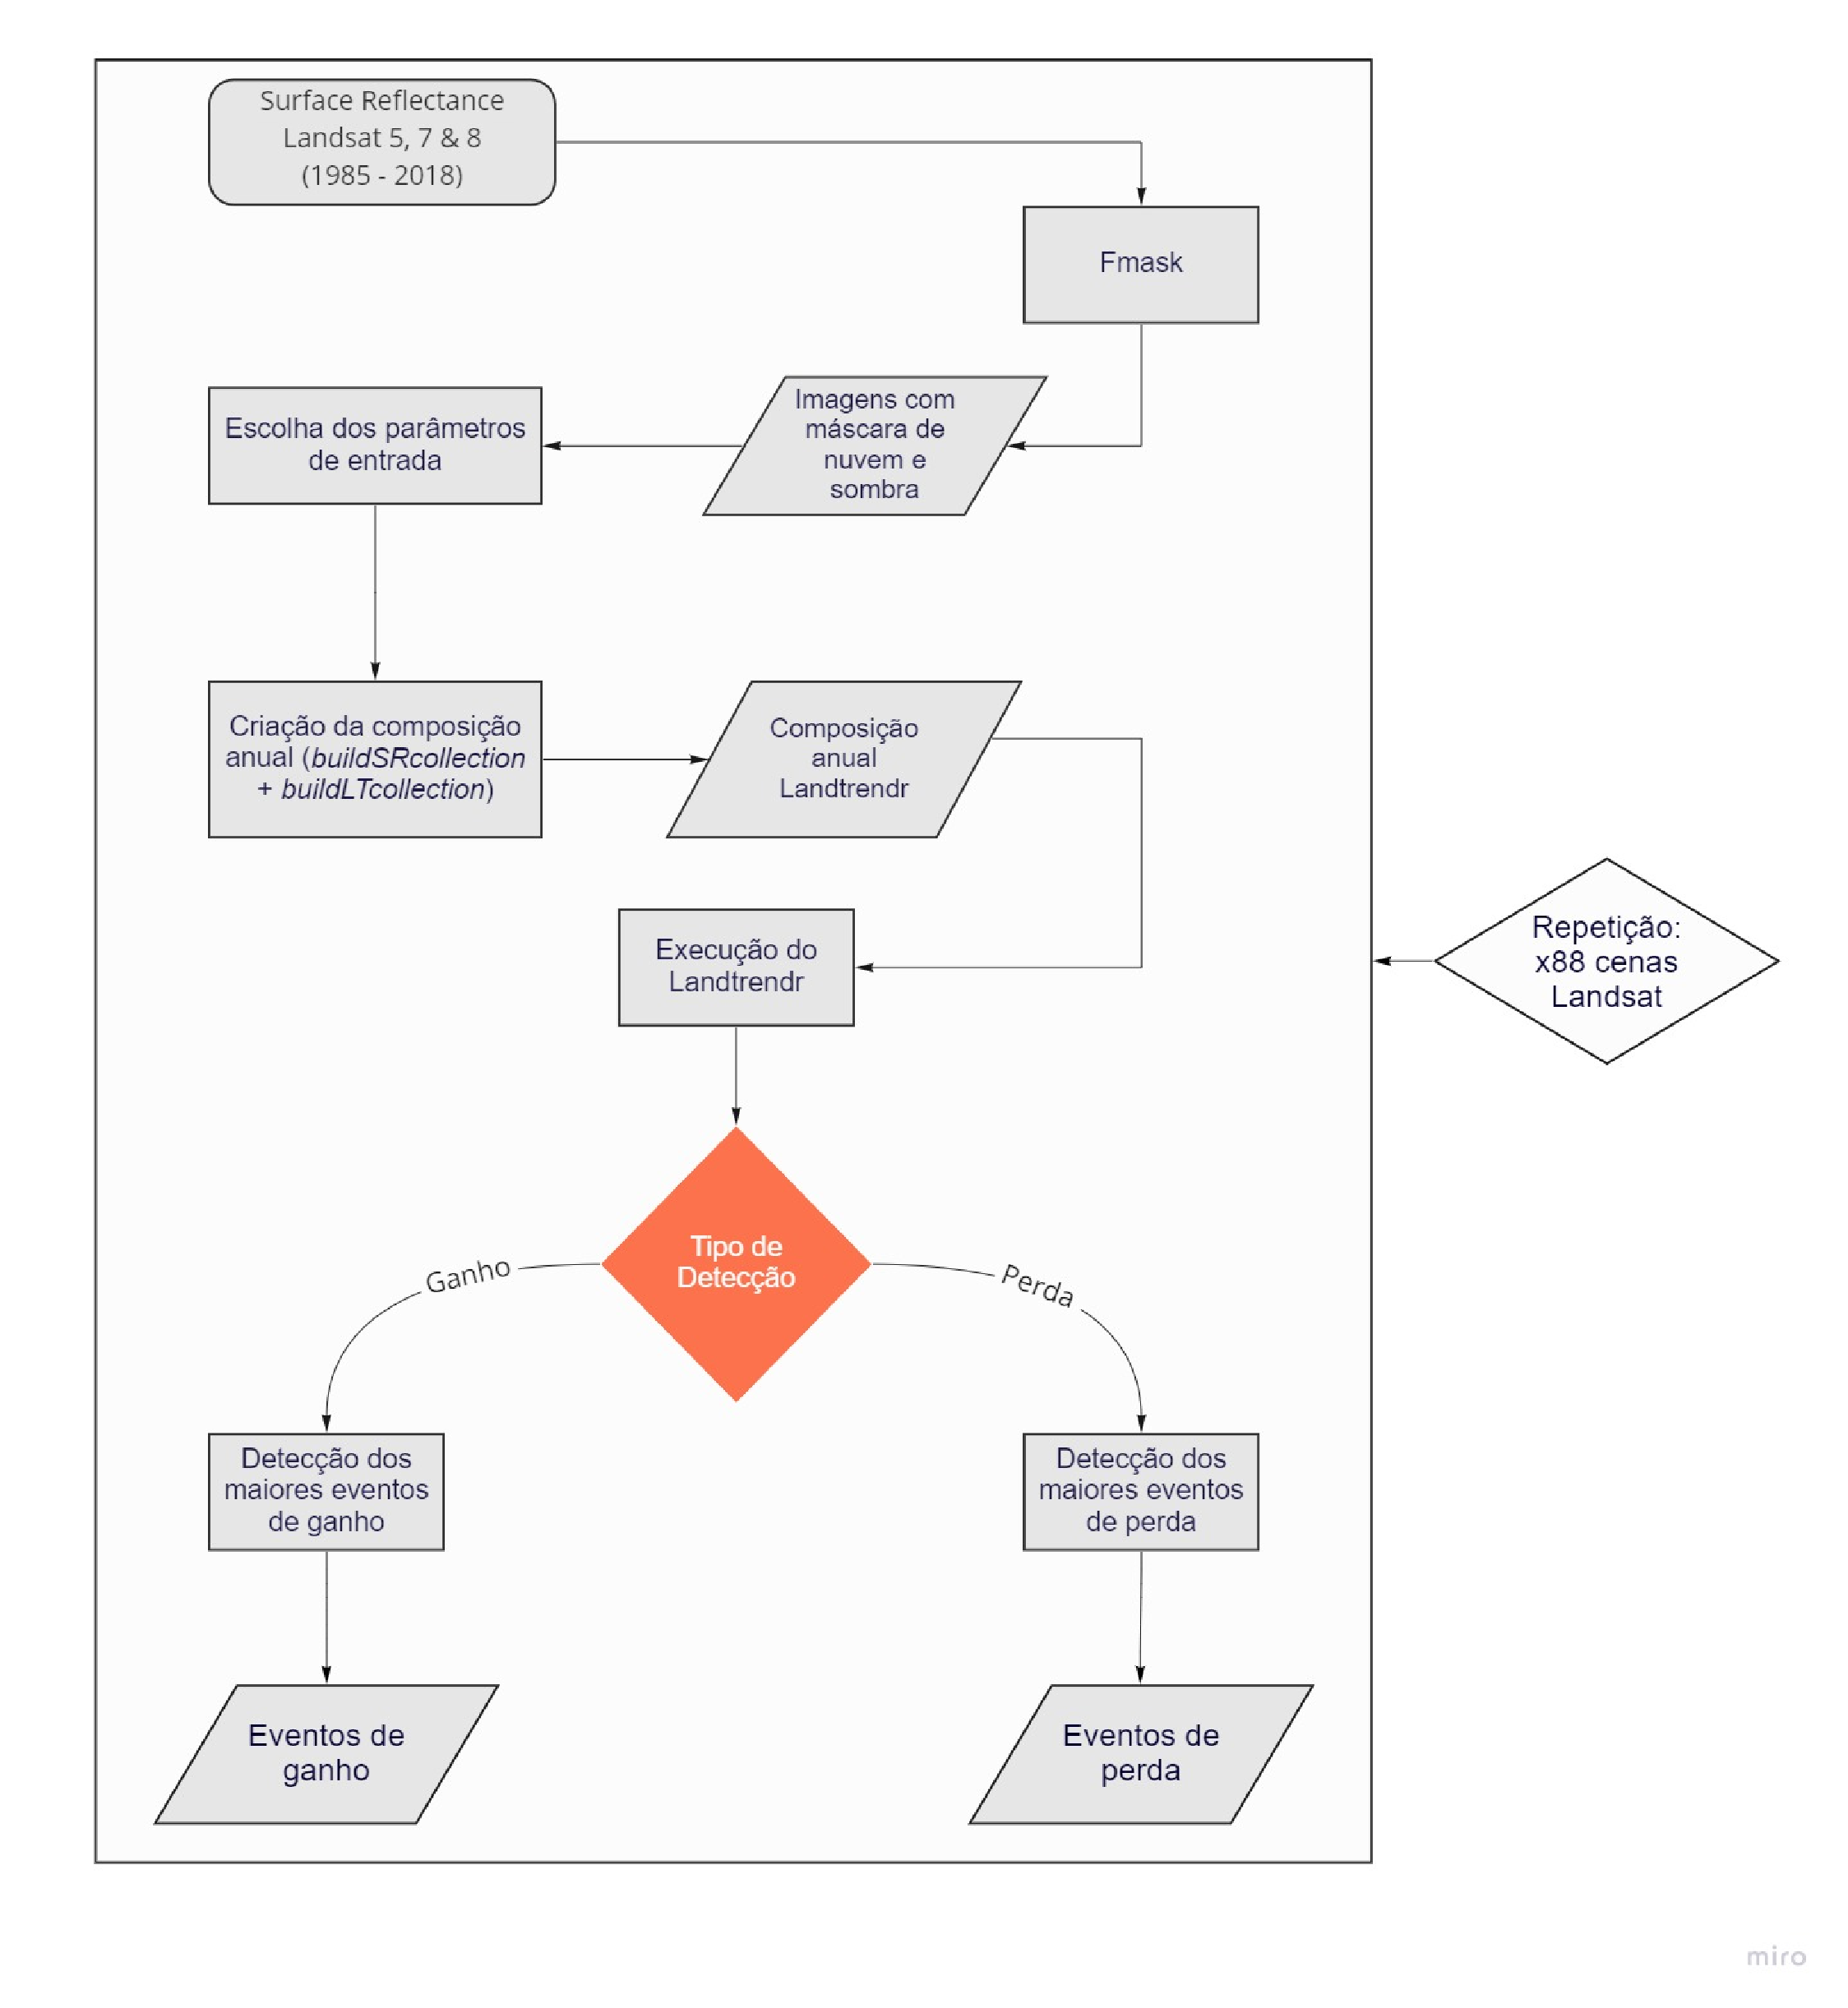
\includegraphics[scale=.5]{images/flowchart_medologia_landtrendr.pdf}
    \caption{Fluxograma do processo de execução do algoritmo Landtrendr}
    \label{fig:flowchart_medologia_landtrendr}
\end{figure}

\subsubsection{Processamento dos cenários de ganho}

\hspace{13pt} Para o cenário de ganho, todos os parâmetros padrão do algoritmo foram mantidos sem nenhum tipo de restrição. Ou seja, \textit{Max Segments} \textbf{6}, \textit{Spike Threshold} \textbf{0.9}, \textit{Vertex Count Overshoot} \textbf{3}, \textit{Prevent One Year Recovery} \textbf{true}, \textit{Recovery Threshold} \textbf{0.25}, \textit{p-value Threshold} \textbf{0.05}, \textit{Best Model Proportion} \textbf{0.75} e \textit{Min Observations Needed} \textbf{6}. Cenários de magnitude (\textit{magnitude}), valor prévio (\textit{previous value}), ano de detecção (\textit{year of detection}), duração (\textit{duration}) e taxa (\textit{rate}) foram gerados e posteriormente pós-processados para limpeza de ruídos e para retirada de valores indesejados. 

Primeiramente, foi gerado uma máscara com todas as áreas pseudo-invariantes entre os anos da análise (1985 - 2018) com o intuito de limpar detecções de mudança muito pequenas. Esta máscara representa todos os pixels que não tiveram nenhum tipo de mudança significativa durante todos os anos da análise, ou seja, áreas que em 1985 já eram consideradas floresta e que se mantiveram praticamente iguais até 2018 (Figura \ref{fig:flowchart_ganho}). 

Inicialmente esta máscara foi desenvolvida utilizando composições anuais de imagens Landsat considerando todos os anos da análise e posteriormente classificadas com o algoritmo Random Forest implementado no pacote MLR \citep{mlr}. No entanto, apesar de apresentar resultados promissores quando a aplicada no mapeamento da área teste na Bacia Hidrográfica do Rio São João, acabou demonstrando problemas quando extrapolada para o resto do bioma e se mostrou uma técnica altamente custosa tanto no tempo de processamento como no tempo de preparação dos dados de entrada \citep{LACERDA2021}. Apesar de não ter sido utilizada como uma máscara neste estudo, a técnica de identificação de áreas pseudo-invariantes utilizando técnicas de aprendizado de máquina pode ser de extrema valia quando aplicada em áreas menores.

Sendo assim, uma abordagem alternativa foi adotada para a criação da máscara para todo o bioma. Camadas de resultado do projeto Mapbiomas v4 foram utilizadas como uma \textit{proxy}. Todas as imagens classificadas para o bioma foram reclassificadas ano a ano em formato binário (floresta [1] e não-floresta [0]) e posteriormente multiplicadas entre si. Um \textit{raster} final binário foi então gerado, onde os pixels com valor 1 representavam áreas que permaneceram como floresta durante todos os anos do estudo e os de valor 0 todos os outros cenários, incluindo além de áreas que presenciaram algum tipo de mudança maior, todas as outras classes mapeadas pelo projeto. Somente pixels da classe floresta (classe número 3) da série 4 foram utilizados. Pixels de classes como floresta plantada foram excluídos assim como o todas as outras. Esta máscara evitou que muitos eventos pudessem ser classificados como ganho, apesar de terem baixa magnitude, já que representavam apenas um processo natural nas florestas já existentes. É importante notar que não estamos nos referindo a áreas de regeneração natural, mas de áreas pseudo-invariantes com variações mínimas durante o período do estudo. 

Além disso, foram mascarados todos os eventos com duração menor ou igual a 4 anos, já que não gostaríamos de incorporar eventos ainda muito recentes ou curtos que poderiam ser identificados como falsos eventos de mudança. O valor mínimo de 5 anos para eventos de ganho ajudou a identificar apenas eventos mais longos que tiveram tempo de apresentar respostas espectrais significativas de recuperação. Com 5 anos a vegetação já passa a apresentar um estágio sucessional característico de floresta secundária inicial \citep{Chazdon2014}. 

\begin{figure}[H]
    \centering
    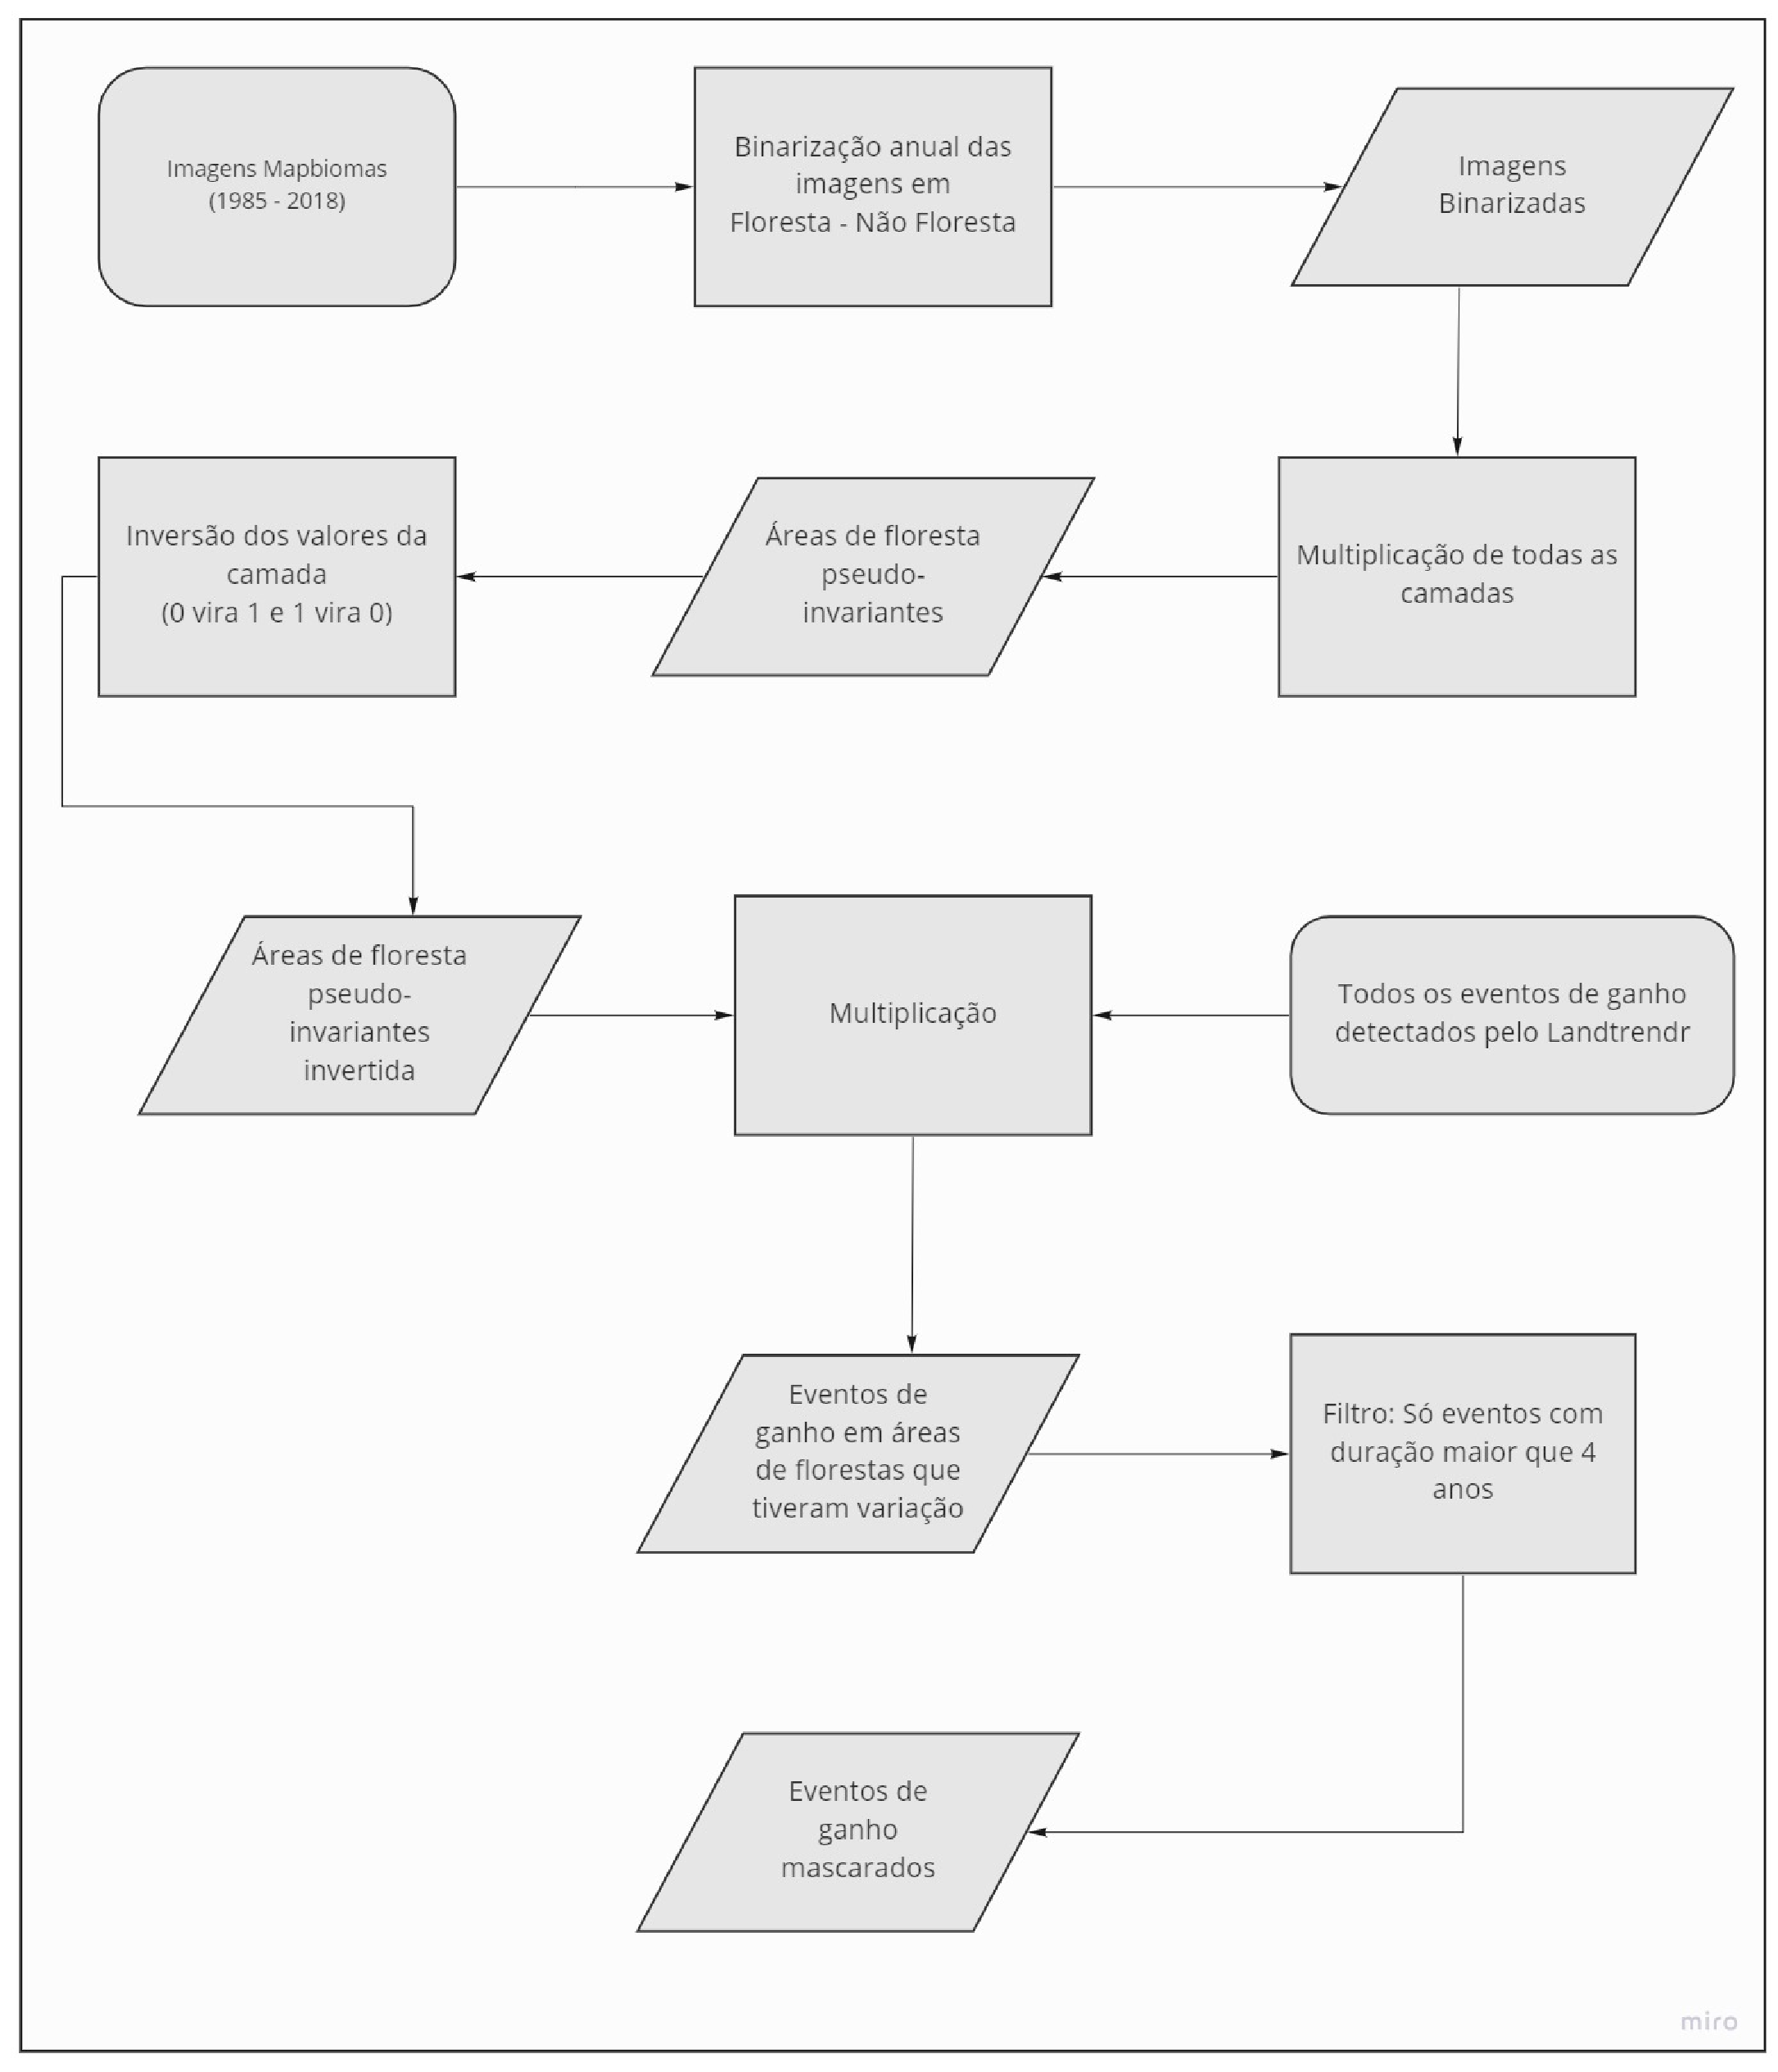
\includegraphics[scale=.4]{images/flow_ganho.pdf}
    \caption{Fluxograma do processo de pós processamento dos dados de ganho}
    \label{fig:flowchart_ganho}
\end{figure}

% figura para ilustrar?

\subsubsection{Processamento dos cenários de perda}
\hspace{13pt} Assim como o cenário de ganho, o processamento do cenário de perda utilizou todos os parâmetros padrões do algoritmo sem nenhum tipo de restrição com o objetivo de realizar limpezas nos resultados obtidos apenas na etapa de pós-processamento. Os mesmos cenários de magnitude (\textit{magnitude}), valor prévio (\textit{previous value}), ano de detecção (\textit{year of detection}), duração (\textit{duration}) e taxa (\textit{rate}) também foram gerados.

No caso das perdas, diferente do cenário de ganho, criou-se uma máscara para garantir que o Landtrendr fosse capaz de detectar mudanças de perda apenas em áreas que foram classificadas como floresta pelo projeto Mapbiomas no ano de 1985. Essa máscara ajudou na não seleção de áreas que nem mesmo tinham sido classificadas como florestas mas que sofreram algum tipo de perda com magnitude grande o suficiente para ser detectada pelo algoritmo. Além disso, uma outra máscara foi gerada para excluir áreas que apesar de terem sido mapeadas em 1985 como floresta e terem sofrido algum tipo de perda significativa, sofreram algum processo de restauração ou regeneração natural ao longo dos anos. Sendo assim, o resultado final para o dado de perdas visou somente a seleção de áreas que tiveram floresta, mas que perderam essa vegetação e não apresentaram nenhum processo de recuperação significativa posterior (Figura \ref{fig:flowchart_perda}).

Diferentemente dos dados de ganho, os dados de perda tem como característica importante a grande variabilidade na duração dos eventos. Sendo assim, utilizou-se a camada de duração para gerar, além das camadas de perda gerais, camadas de perda com duração igual a um ano e camadas com duração superior à um ano. Esta diferenciação é importante para que possamos identificar eventos de perda rápida, sejam eles de natureza antrópica ou natural, normalmente associados à cortes rasos ou queimadas.

\begin{figure}[H]
    \centering
    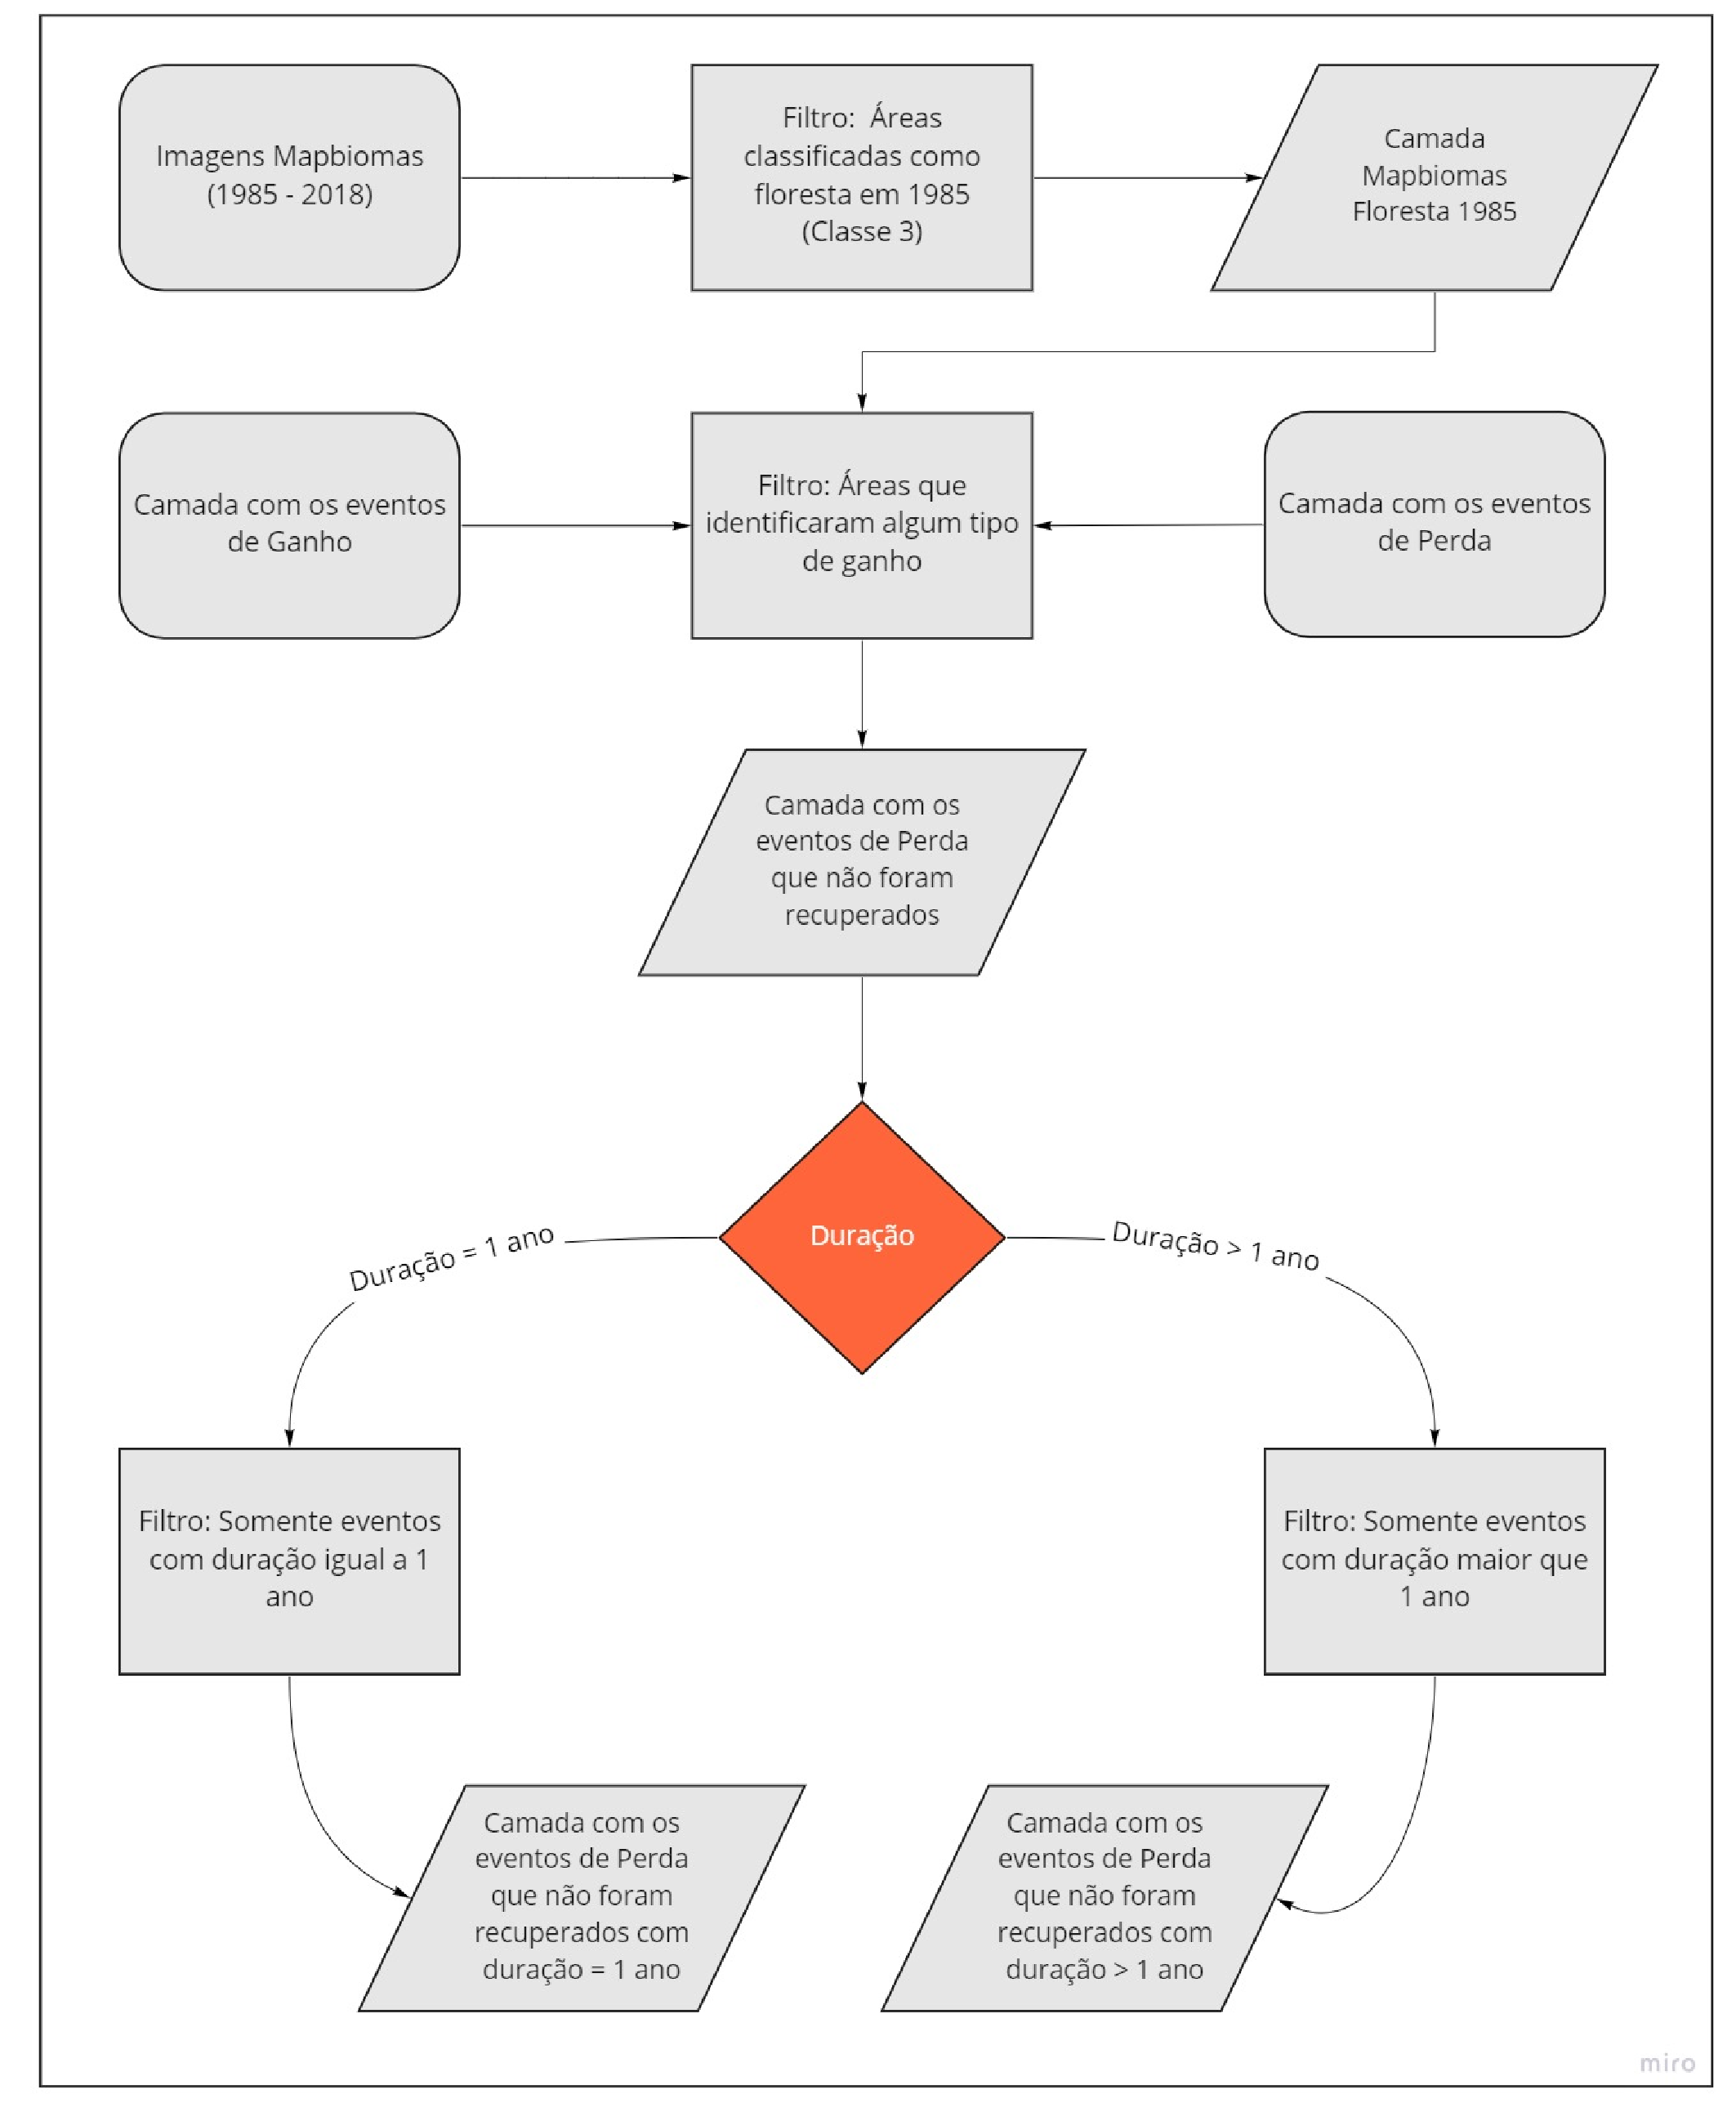
\includegraphics[scale=.4]{images/flow_perda.pdf}
    \caption{Fluxograma do processo de pós processamento dos dados de perda}
    \label{fig:flowchart_perda}
\end{figure}

\subsubsection{Escolha dos limiares para a filtragem dos eventos de mudança}
\hspace{13pt} Para além da filtragem das áreas de interesse, é interessante que, em alguns casos, uma segunda etapa de filtragem seja realizada para garantir que mesmo nas áreas de interesse, os pixels detectados como eventos de mudança pelo algoritmo estejam realmente dentro do esperado e façam sentido dentro do contexto da análise. 

Para isso, o Landtrendr possui a possibilidade de especificação de parâmetros de filtragem (\textit{Change Mapping Parameters}). Através da especificação desses parâmetros é possível realizar, já na execução do algoritmo, a filtragem dos eventos de acordo com a magnitude, duração e valor prévio (\textit{Pre-Dist Value}) do evento. 

É possível, por exemplo, a filtragem de todos os maiores eventos de perda que possuam duração maior que 4 anos, com magnitude maior que 400 e valor prévio maior que 600. No entanto, ao aplicar o algoritmo no contexto da Mata Atlântica, foi possível observar que a variabilidade de contextos espaciais pode implicar em muitos casos na filtragem de eventos indesejáveis, ou seja, falso-negativos. Apesar da facilidade apresentada pela implementação do algoritmo, fica evidente a necessidade da condução de testes para o maior entendimento da região a ser mapeada antes da aplicação de qualquer filtro deste tipo. A possibilidade de uso de filtros prévios acabam beneficiando apenas situações onde a área a ser mapeada foi previamente estudada ou em situações onde o resultado deve se restringir apenas a algumas características específicas.

Para este estudo, um filtro especificando um limiar para os eventos de perda era necessário. Muitos eventos com pouca magnitude foram detectados, representando áreas que houveram perdas, mas não significativas o suficiente ao longo da série para representar uma real mudança no uso e cobertura do solo.   

Sendo assim, testes foram realizados tanto para áreas de florestas ombrófilas densas quanto estacionárias semideciduais, já que era possível que o valor do limiar pudesse ser diferente de acordo com a fitofisionomia estudada. Cem amostras foram coletadas para cada fitofisionomia de floresta como também para áreas de pasto dentro de cada contexto. O valor médio de NDVI encontrado para áreas de floresta estacionária foi de 0.80 e ombrófila de 0.86. Já para áreas de pasto, o valor médio foi de 0.61. Ou seja, uma diferença média de mais de 0.2 ou mais de 200 de magnitude entre áreas de floresta e de pasto. Além disso, a média geral da magnitude dos eventos de perda na Mata Atlântica foi de 225, o que corroborou para o resultado comparativo. Comparando-se as médias das amostras de floresta ombrófila com amostras de pasto, o p-valor obtido foi de 1.599e-11, já para a comparação com as amostras de florestas estacionárias o valor do teste-t foi de 2.495e-7. Ou seja, independente da fitofisionomia, ambas as situações apresentaram diferença estatisticamente significativa em suas médias.

No entanto, este valor de limiar encontrado não foi suficiente para ser utilizado como máscara para as análises de perda devido a um alto desvio padrão encontrado nos valores de magnitude (média de 123). Foi observado que muitas áreas que já apresentavam um certo grau de degradação já possuíam números próximos de áreas de pasto com valor de magnitude próximas de 150. Para não excluirmos estas áreas do resultado, optou-se então por realizar a filtragem utilizando máscaras baseadas em camadas previamente geradas pelo projeto Mapbiomas v4 como descrito anteriormente.

Para áreas de estudos que não possuam mapeamentos de uso e cobertura anuais, a filtragem pela magnitude pode sim ser uma boa prática e forma de limpeza dos resultados finais. Além disso, uma solução híbrida também é possível. Entretanto, para áreas extensas como a Mata Atlântica, a especificação de uma constante de filtragem pode ser arriscada devido a alta variabilidade de contextos ecológicos e de interferência antrópica na região.

\subsection{Resultados e Discussões}

\hspace{13pt} Os resultados para os cenários de perda e ganho foram aglomerados (\textit{merge}) em imagens únicas abrangendo todo o bioma para cada cenário. Com isso, foi possível compilar os resultados analisando o contexto geral da região e posteriormente transformando os arquivos matriciais em arquivos vetoriais. Essa transformação foi necessária para facilitar a visualização através de mapas de calor (\textit{heatmaps}). Os resultados foram transformados para um sistema de referência de área igual ideal para analises de áreas de grandes extensões. Neste caso específico foi utilizado a projeção de Albers, mais especificamente a projeção \textit{South America Albers Equal Area Conic} (ESRI: 102003). 

\subsubsection{Validação}

\hspace{13pt} Entender os erros gerados em um processo de detecção para uma área extensa como a Mata Atlântica é complicado e requer certo exercício de individualização de cenários já que estamos tratando de dinâmicas dissemelhantes. Entendendo isso, o processo de validação teve de ser executado de forma individual para cada fitofisionomia estudada. A ideia foi buscar entender o comportamento, as semelhanças e as discrepâncias entre as diferentes fitofisionomias.

O processo de validação de séries temporais possui algumas semelhanças com o processo tradicional, mas também algumas diferenças significativas que acabam impactando de forma direta o planejamento da execução. Assim como na validação de uma única data, é esperado que o especialista faça a interpretação visual das amostras. No entanto, na validação de séries temporais a interpretação necessita de uma série temporal de imagens, que a depender da resolução temporal, impossibilita o uso de imagens de mais alta resolução, como no caso desse estudo. Além disso, é interessante que se possua alguma forma de visualização de toda a série de forma prática, algo não implementado de forma padrão na grande maioria dos SIG disponíveis. O que se tem muitas vezes é apenas uma visualização em forma de gráfico em duas dimensões dos valores da série para cada pixel, sem muita informação sobre o contexto local. Devido a estas necessidades que ferramentas como o TimeSync foram desenvolvidas \citep{COHEN20102911}.

O TimeSync possui uma interface gráfica  apropriada para a visualização de toda a série tanto em forma de imagens quanto de gráficos (Figura \ref{fig:loss_22_bhrsj_graph} \& \ref{fig:loss_22_bhrsj_imgs}). O TimeSync também utiliza arquivos no formato do Microsoft Access tanto para a configuração do programa quanto para o registro final da validação. O \textit{software} visa a análise de séries anuais, já que foi desenvolvido para ser utilizado como um facilitador do processo de validação dos resultados do Landtrendr. No entanto, pode sim ser utilizado para a validação de resultados de outros algoritmos, desde que sejam derivados de séries anuais.

\begin{figure}[H]
    \centering
    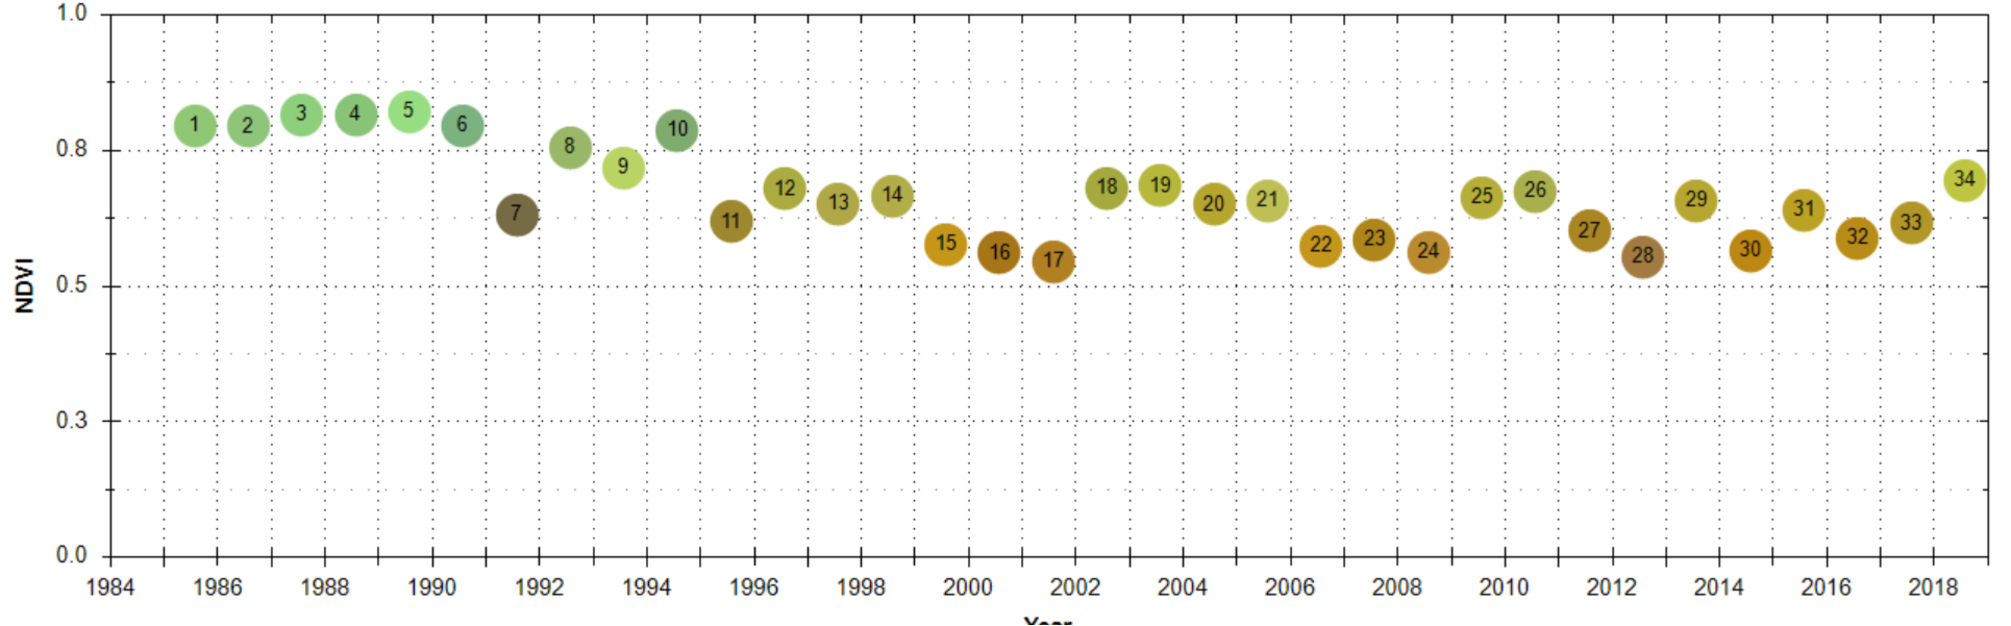
\includegraphics[scale=.4]{images/loss_22_bhrsj_graph.pdf}
    \caption{Visualização dos valores de NDVI para cada ano. A cor dos pontos segue a mesma coloração obtida pelo pixel na imagem, o que ajuda na interpretação visual dos eventos. Na imagem, podemos ver um evento de perda.}
    \label{fig:loss_22_bhrsj_graph}
\end{figure}

\begin{figure}[H]
    \centering
    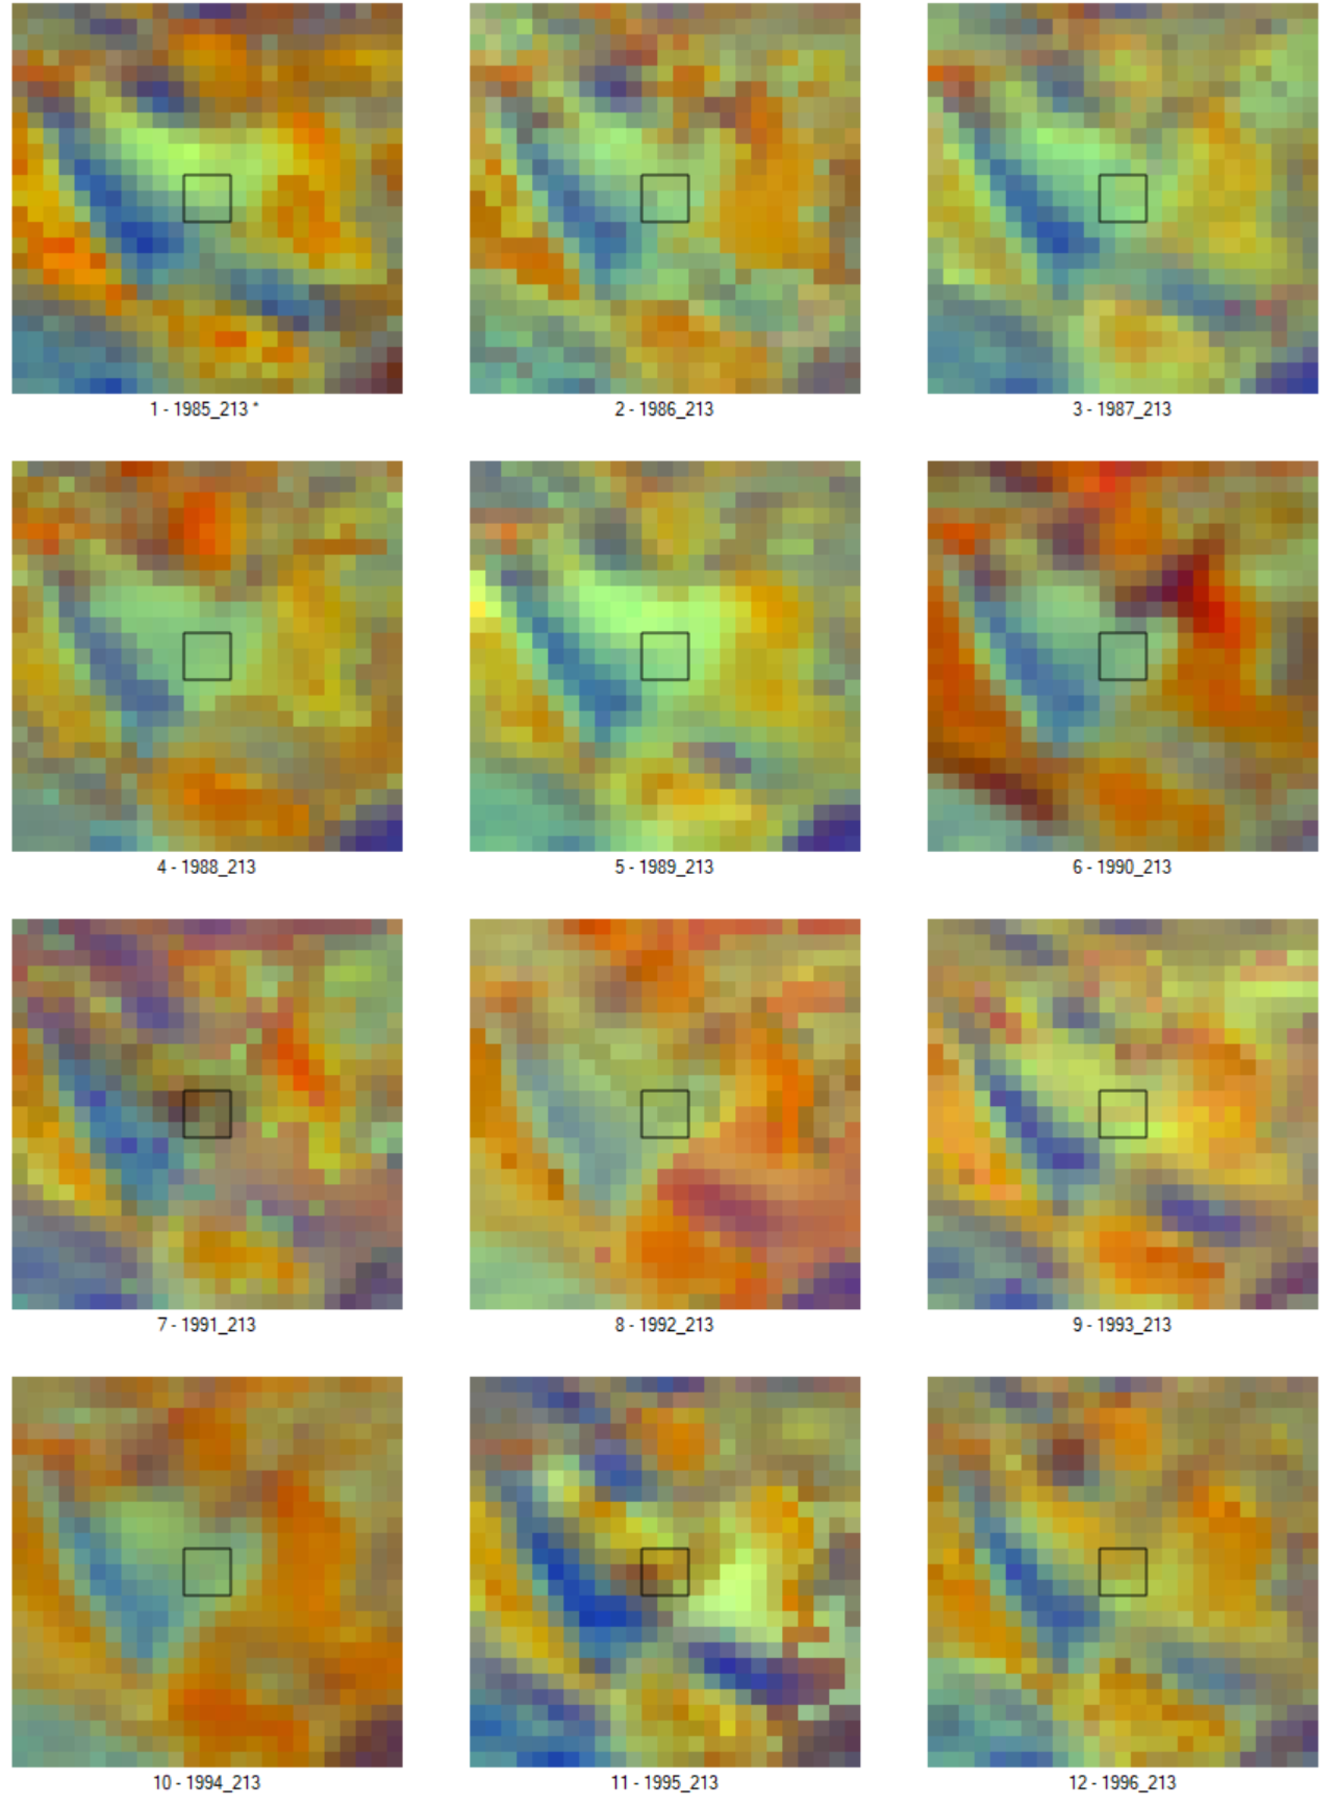
\includegraphics[scale=.5]{images/loss_22_bhrsj_imgs.pdf}
    \caption{TimeSync Image Viewer. Evento de perda na bacia hidrográfica do rio São João. Cada imagem representa o mesmo pixel/local para cada ano do estudo.}
    \label{fig:loss_22_bhrsj_imgs}
\end{figure}

Desde a implementação do Landtrendr no GEE, o TimeSync ainda possui scripts em Python que visam facilitar a exportação de séries temporais do GEE para um ambiente \textit{offline}. Esta etapa é essencial, já que diferente da versão para ENVI/IDL do Landtrendr, no GEE, toda a etapa de preparação dos dados de entrada e de seu processamento são feitos na nuvem de forma quase que automática pelo próprio algoritmo. Como a validação tem de ser feita em ambiente \textit{offline}, é necessário baixar a série inteira ou pedaços da mesma para a realização deste processo. 

No caso da validação de uma área extensa como a da Mata Atlântica, apenas pedaços da série foram exportados já que o processo de exportação de toda a área seria muito demorado, custando algumas horas para a exportação de áreas com apenas algumas centenas de $ km^2 $. Devemos considerar também que a exportação de toda a série para uma área extensa em resolução espacial de 30m necessitaria de excessivo espaço para armazenamento, sendo incoerente com a proposta inicial de processamento de grande escala e com baixo custo. 
Sendo assim, uma área de teste foi escolhida para cada fitofisionomia estudada.

Para cada área selecionada, pontos aleatórios distribuídos de forma estratificada foram gerados para três classes distintas: Ganho, Perda e  pseudo-invariância/Outros. A classe de Pseudo-invariância/Outros foi criada para comportar todos os pontos que na verdade não eram de interesse da análise de detecção de mudanças. Sejam por serem áreas que se mantiveram constante ao longo dos anos estudados ou porque foram mascaradas por serem áreas urbanas, áreas naturais não vegetada ou qualquer outra classe de não interesse. Para cada classe foram gerados 100 pontos, totalizando 300 pontos de validação para cada fitofisionomia, uma soma total de 900 pontos. Além disso, mais 300 pontos (100 por classe) foram validados para a Bacia Hidrográfica do Rio São João com o intuito, assim como no estudo sobre a banda CSNR, verificar possíveis variações no resultado do algoritmo para regiões geograficamente distantes mas fitofisionomicamente similares.

Nas áreas de floresta ombrófila densa, os resultados mostraram uma acurácia de 90\% e um kappa de 0.85. Já nas áreas de vegetação ombrófila mista, obtivemos uma acurácia de 88\% com um kappa de 0.82. Finalmente, nas áreas de vegetação estacional semidecidual, a acurácia, como esperado, foi um pouco menor ficando em 84\% e com kappa 0.76. Apesar da diferença aparente entre regiões ombrófilas e estacionais, todas as regiões obtiveram resultados considerados altos, e portanto, satisfatórios, mostrando que ao utilizar composições anuais essas diferenças causadas pelas dinâmicas estacionais acabem se diluindo. Não foram detectadas diferenças significativas entre os erros de comissão e omissão. As mesmas mantiveram resultados semelhantes em todas as fitofisionomias analisadas.  
Esta diluição causada pela composição de séries anuais fica ainda mais clara quando os testes para a região adicional da Bacia Hidrográfica do Rio São João foram analisados. Para a bacia, uma região classificada como ombrófila densa, foi obtido uma acurácia de 85\% e kappa de 0.77, o que estaria muito mais próximo dos resultados obtidos para a região estacional do que das ombrófilas. Espera-se que os resultados obtidos por fitofisionomia possam contribuir para o entendimento da característica mais homogênea dos estudos que tem como dado de entrada composições derivadas de uma coleção densa de imagens. Além disso, uma validação considerando todas as regiões estudadas foi feita, obtendo um valor de acurácia global de 86.7\% e kappa de 0.8. 

Estes resultados demonstraram um excelente resultado obtido pelo algoritmo e confirmam seu potencial para aplicação em áreas tropicais extensas.

\subsubsection{Plataforma para visualização dos resultados}

\hspace{13pt} Uma das dificuldades encontradas na análise de áreas extensas como a Mata Atlântica está na representação dos resultados, principalmente em escalas derivadas de resoluções espaciais médias como no caso das imagens Landsat. A criação de mapas de calor e criação de estatísticas zonais acabam servindo para uma análise mais geral das regiões e até mesmo em nível de município, mas limita uma análise mais pontual, local.

A plataforma do Google Earth Engine (GEE) disponibiliza a possibilidade de criação de uma interface gráfica através da própria API, possibilitando a publicação de resultados obtidos na plataforma ou de dados externos importados para seu ambiente através da criação de um \textit{website}. Esta funcionalidade possibilita a divulgação interativa de forma prática e rápida de grande quantidade de dados. Sem esta infraestrutura, o compartilhamento dos dados resultantes de análises na plataforma teriam de ser feito de forma tradicional, através do \textit{download} dos dados da plataforma e posterior \textit{upload} em serviços de hospedagem na nuvem. Para dados como os resultados obtidos nesta análise esta opção se mostrou essencial, já que os arquivos resultantes são grandes e demandam poder computacional significativo para uma visualização sem engasgos. 

A criação de uma aplicação web utilizando o GEE pode ser feita de forma relativamente simples através da própria interface gráfica. O desenvolvimento da interface gráfica deve ser realizada utilizando a API JavaScript, que possui documentação extensa no próprio \textit{website} oficial. Os dados que serão visualizados devem estar conectados a sua conta do GEE e compartilhados de forma aberta. Após o link dos dados com a interface, é possível fazer a publicação através do botão "App". A plataforma leva alguns minutos para subir a aplicação final e gerar um link compartilhável Figura (\ref{fig:ltr_gee_ui_atlatic_forest}). 

Neste caso, o código para a aplicação ainda foi registrado na plataforma Zenodo com o objetivo de gerar um DOI (10.5281/zenodo.6481487). O código fonte para a aplicação pode ser acessado aqui: https://github.com/sacridini/ui\_gee\_ltr\_mata\_atlantica. A visualização das principais camadas geradas neste trabalho (perda, perda rápida, perda longa e ganho) podem ser acessadas através deste link: https://elacerda.users.earthengine.app/view/atlantic-forest-landtrendr. 

\begin{figure}[H]
    \centering
    \includegraphics[scale=.3]{images/ltr_gee_ui_atlatic_forest.pdf}
    \caption{Página principal da aplicação web para visualização dos resultados de mudança na Mata Atlântica}
    \label{fig:ltr_gee_ui_atlatic_forest}
\end{figure}

\subsubsection{Resultados para os eventos de perda na Mata Atlântica}

\hspace{13pt} Somando-se todos os eventos de perda detectados pelo algoritmo após as filtragens das áreas de interesse, houveram ao longo de todos os anos da análise 61.167.796 de pixels com uma perda média de magnitude de 225 ou diminuição de 0.225 no índice NDVI. Isso equivale a uma área total de pouco mais de 55 mil $ km^2 $ de florestas que sofreram perdas significativas no bioma e que não foram recuperadas após a supressão.

O resultado mais abrangente envolvendo todos os eventos de perda do bioma pode ser visualizado na (Figura \ref{fig:heat_loss_masked85_maskedgain}). A maior aglomeração de eventos de perda está localizada principalmente entre os estados do Paraná e Santa Catarina e no estado da Bahia. Nos outros estados o mapa de calor mostra uma distribuição mais homogênea dos eventos ao longo do território. 

\begin{figure}[H]
    \centering
    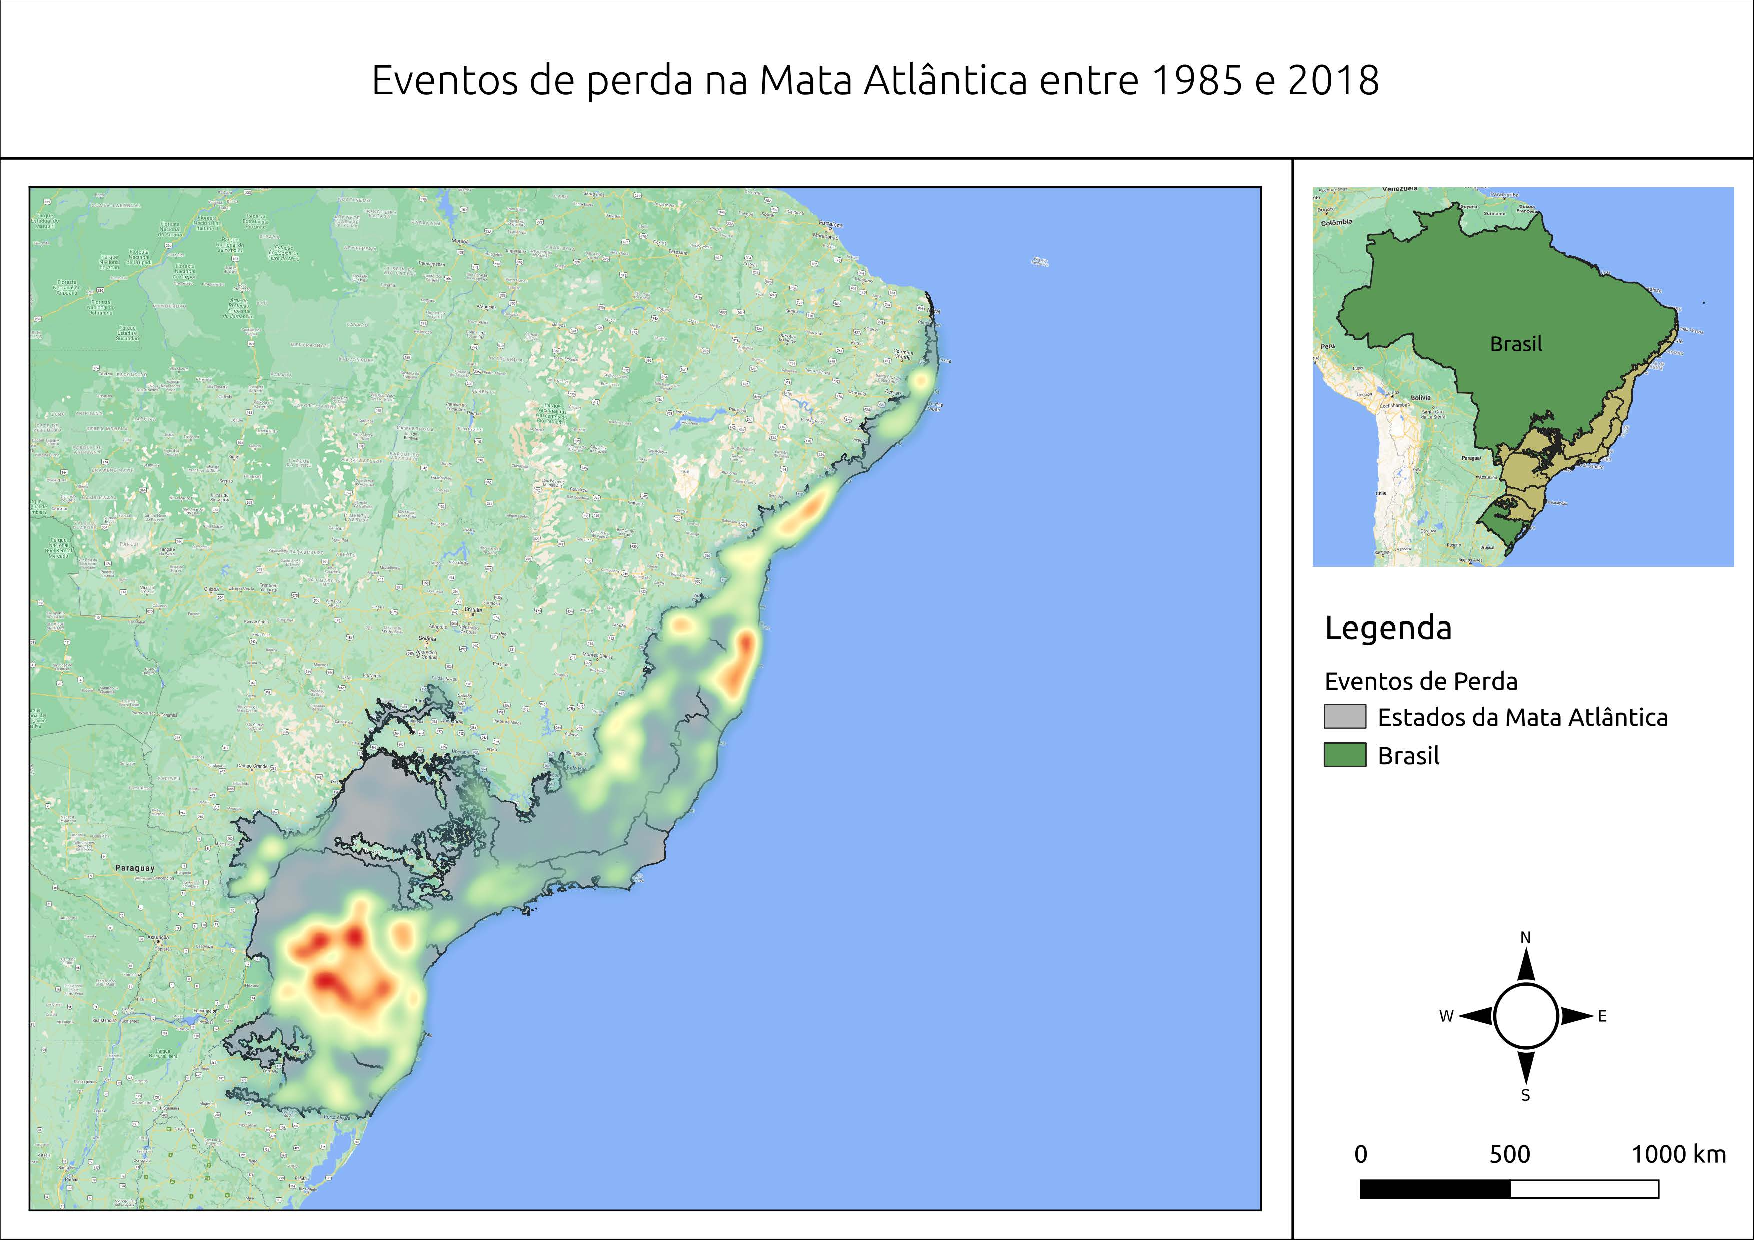
\includegraphics[scale=.5]{images/heatmap_loss_masked85_maskedgain.pdf}
    \caption{Todos os eventos de perda na Mata Atlântica entre 1985 e 2018.}
    \label{fig:heat_loss_masked85_maskedgain}
\end{figure}

\subsubsection{Os eventos de ganho na Mata Atlântica}

\hspace{13pt} Somando-se todos os eventos de ganho detectados pelo algoritmo e após as filtragens necessárias, houveram ao longo de todos os anos da análise 68.869.908 de pixels com um ganho médio de 197 ou aumento de 0.197 no índice NDVI. Isso equivale a uma área total de aproximadamente 62 mil $ km^2 $ de florestas que sofreram ganhos significativos. Como discutido na sessão 3.2.4, áreas de florestas pseudo-invariantes não foram consideradas, sendo assim, esta área representa um ganho real de área verde dentro do bioma. 

Na Figura \ref{fig:heat_gain}, podemos observar que o ganho de áreas no bioma de deu de forma bem mais homogênea que as áreas de perda. Apenas algumas áreas de aglomeração podem ser visualizados como no sul do Rio Grande do Sul, Espírito Santo, sul de Pernambuco, São Paulo e Minas Gerais.

\begin{figure}[H]
    \centering
    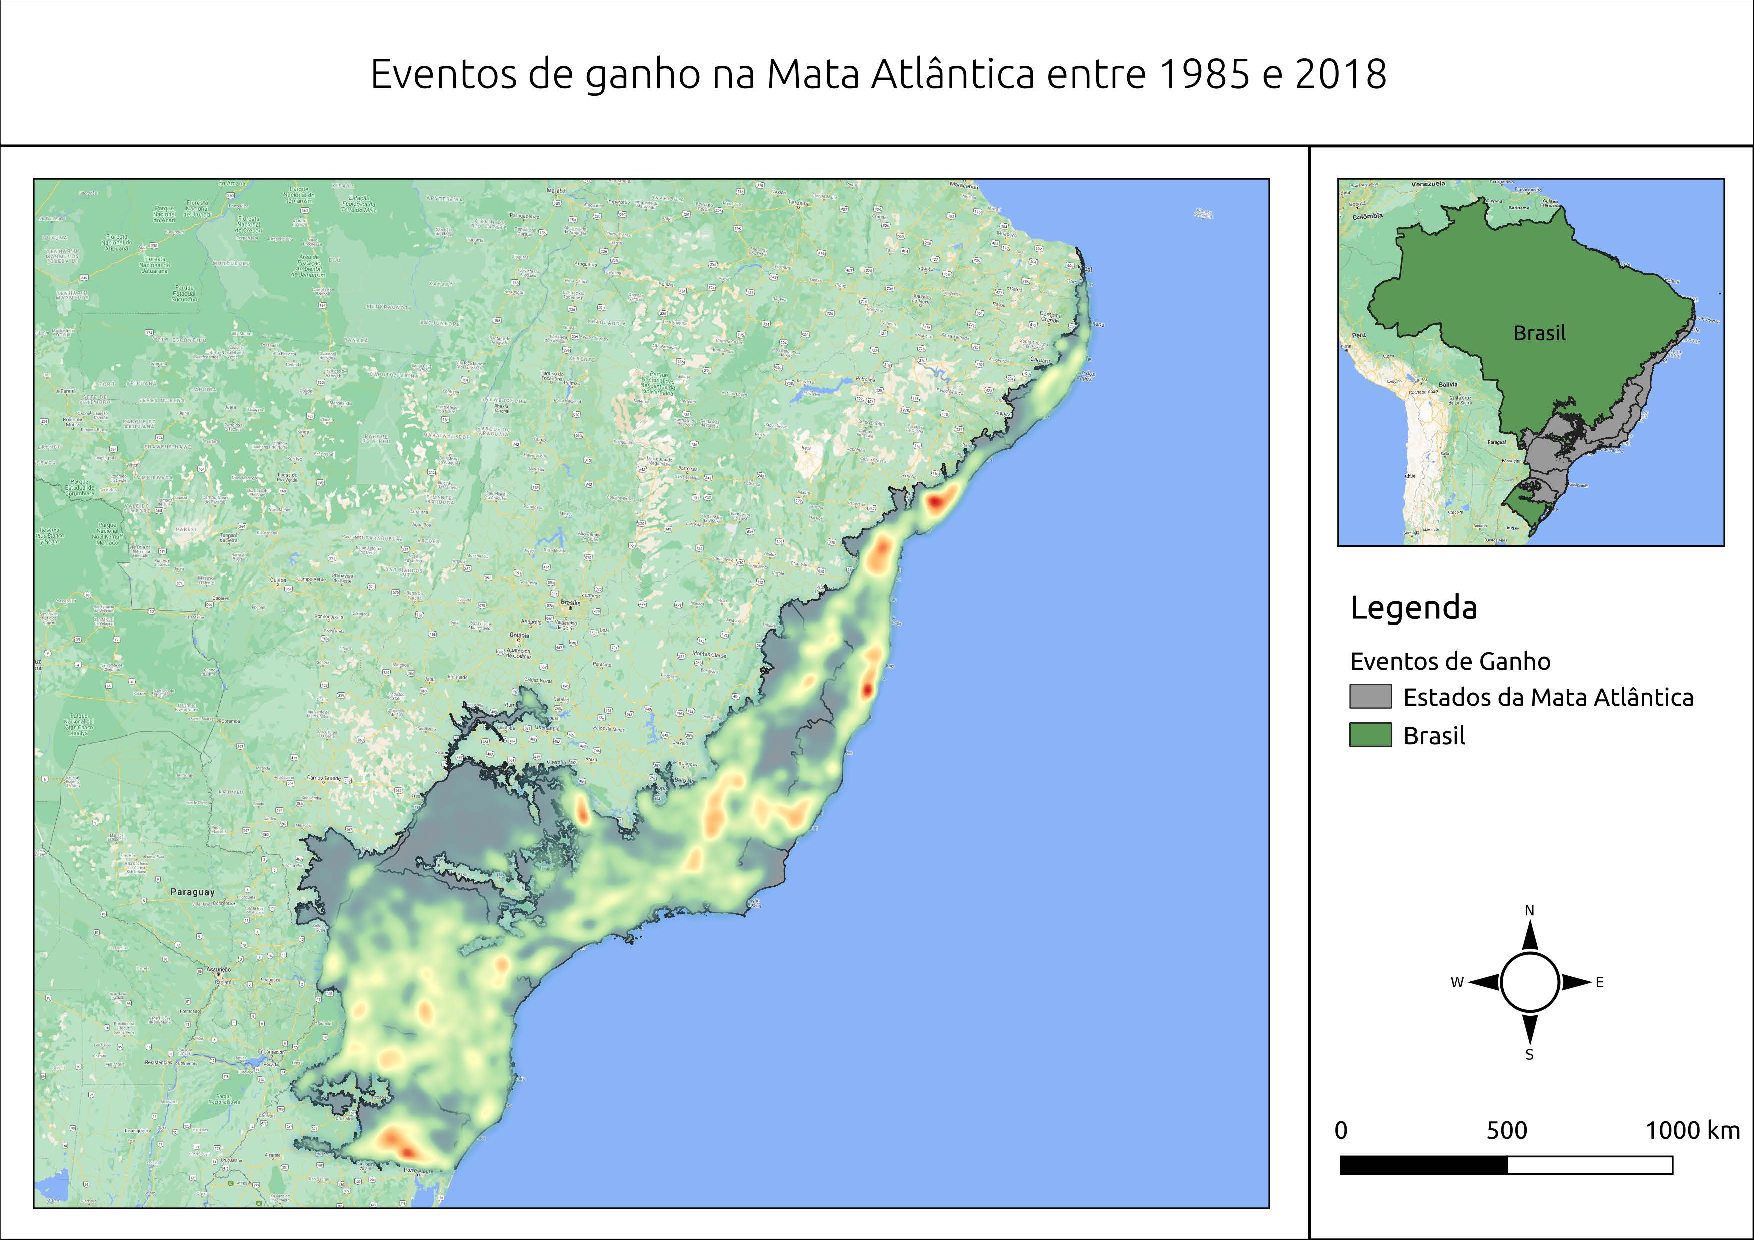
\includegraphics[scale=.5]{images/heatmap_gain_masked18_dur_gt4_inv_for.pdf}
    \caption{Eventos de ganho entre 1985 e 2018.}
    \label{fig:heat_gain}
\end{figure}

\subsection{Conclusão}

\hspace{13pt} Podemos observar através deste estudo que o algoritmo Landtrendr apresentou resultado bastante satisfatório quando aplicado à áreas extensas de floresta tropical. Diferente de estudos realizados anteriormente, foi possível observar o comportamento do algoritmo quando aplicado a diferentes fitofisionomias. Os resultados apresentados são coerentes com os apresentados por programas de mapeamento sistemáticos com o Mapbiomas, mas contribuiu para uma melhor qualificação das mudanças ocorridas no bioma ao longo dos 33 anos da análise. 

Este estudo contribui ainda para o desenvolvimento do conhecimento sobre a aplicação de técnicas de detecção de mudança baseado em trajetórias em um contexto ecológico complexo e fragmentado como o da Mata Atlântica em meso-escala. A incorporação de ferramentas de processamento de dados espacias em infraestruturas computacionais interconectadas demonstra através de trabalhos como este, mais uma vez, sua potencialidade. Não só na clara capacidade extraordinária de processamento como na qualidade das ferramentas disponíveis para análise dos dados. Observando os resultado obtidos, acreditamos que a implementação do Landtrendr para a plataforma Google Earth Engine poderá contribuir para futuras análises, sejam elas locais ou para áreas extensas, utilizando assim todo o potencial de processamento disponível.
% Estes fatores foram essenciais para contarmos esta parte recente e importante da história da Mata Atlântica. 